%%%%%%%%%%%%%%%%%%%%%%%%%%%%%%%%%%%%%%%%%%%%%%%%%%%%%%%%%%%%%%%%%%%%%%%%%%%%%%%%
% Template for TISMIR Papers
% 2017 version, based on previous ISMIR conference template
%%%%%%%%%%%%%%%%%%%%%%%%%%%%%%%%%%%%%%%%%%%%%%%%%%%%%%%%%%%%%%%%%%%%%%%%%%%%%%%%

\documentclass{article}

%%%%%%%%%%%%%%%%%%%%%%%%%%%%%%%%%%%%%%%%%%%%%%%%%%%%%%%%%%%%%%%%%%%%%%%%%%%%%%%%
% Sample Document LaTeX packages
%%%%%%%%%%%%%%%%%%%%%%%%%%%%%%%%%%%%%%%%%%%%%%%%%%%%%%%%%%%%%%%%%%%%%%%%%%%%%%%%
\usepackage[utf8]{inputenc}
% To remove the line numbers for the camera-ready version of your paper, remove
% the `review` option from the tismir package
\usepackage[review]{tismir}
\usepackage{amsmath}
\usepackage{hyperref}
\usepackage{url}
\usepackage{graphicx}
\usepackage{booktabs}
\usepackage{lipsum}
\usepackage{subcaption} 

\graphicspath{ {./figures/} }
\urlstyle{same}

%%%%%%%%%%%%%%%%%%%%%%%%%%%%%%%%%%%%%%%%%%%%%%%%%%%%%%%%%%%%%%%%%%%%%%%%%%%%%%%%
% Title and Author information
%%%%%%%%%%%%%%%%%%%%%%%%%%%%%%%%%%%%%%%%%%%%%%%%%%%%%%%%%%%%%%%%%%%%%%%%%%%%%%%%

\title{Power to the People!  Assigning Popular Music Genres Based on Listeners' Perspective Using a Genre Tree Approach}
%

\author{Anonymous}
% \author{%
% Markus Radke\thanks{Audio Communication Group, Technische Universität Berlin, Einsteinufer 17c, 10587 Berlin, Germany} %
% ~and Steffen Lepa\protect\footnotemark[1]}

\date{}

%%%%%%%%%%%%%%%%%%%%%%%%%%%%%%%%%%%%%%%%%%%%%%%%%%%%%%%%%%%%%%%%%%%%%%%%%%%%%%%%
% Additional Paper Information
%%%%%%%%%%%%%%%%%%%%%%%%%%%%%%%%%%%%%%%%%%%%%%%%%%%%%%%%%%%%%%%%%%%%%%%%%%%%%%%%

\type{research}

% Citation in First Page
\authorref{Anonymous}
% \authorref{Radke,~M. and Lepa,~S.}

%
% (Optional)
% \journalyear{2017}
% \journalvolume{V}
% \journalissue{N}
% \journalpages{xx--xx}
% \doi{xx.xxxx/xxxx.xx}

% Remaining Pages (Optional)
\authorshort{Anonymous} 
% \authorshort{Radke, M. and Lepa, S.} 
\titleshort{Power to the People! Assigning Popular Music Genres}

%%%%%%%%%%%%%%%%%%%%%%%%%%%%%%%%%%%%%%%%%%%%%%%%%%%%%%%%%%%%%%%%%%%%%%%%%%%%%%%%
% Document Content
%%%%%%%%%%%%%%%%%%%%%%%%%%%%%%%%%%%%%%%%%%%%%%%%%%%%%%%%%%%%%%%%%%%%%%%%%%%%%%%%

\begin{document}

%%%%%%%%%%%%%%%%%%%%%%%%%%%%%%%%%%%%%%%%%%%%%%%%%%%%%%%%%%%%%%%%%%%%%%%%%%%%%%%%
% Abstract
%%%%%%%%%%%%%%%%%%%%%%%%%%%%%%%%%%%%%%%%%%%%%%%%%%%%%%%%%%%%%%%%%%%%%%%%%%%%%%%%

\twocolumn[{%
%
\maketitleblock
%
\begin{abstract}
Despite popularity of playlists on streaming platforms, music genres still remain a primary organizational tool among listeners, stakeholders, and researchers. Yet both `correct' genre labels for popular music exemplars and structure of genre taxonomies are often contested. Nevertheless, questionable categorical genre assignments form the basis of many music genre recognition models in MIR and recommender systems research as well as in musicological basic research on music preferences and functions, raising concerns about reliability, validity, and comparability of results. In contrast, popular music studies have long emphasized the listener-dependent nature of genre assignments. In other words: Genre assignment may be considered a matter of majority voting within a listener community. So why not make a virtue of necessity? We present a new methodology for constructing hierarchical genre trees from \textit{MusicBrainz} folksonomy genre votes and demonstrate feasability of this approach  for 167,762 tracks listened to in Germany across the past 50 years. The resulting Community Music Genre Tree for popular music in Germany (COMGET-G) comprises 234 genres—interesting for cultural analyses, but probably too detailed for many applied research tasks. We address this by presenting an additional algorithm for folding such trees to a desired number of genre categories for any research problem (FOLDCAT). For automatic category assignment of music tracks still lacking community votes, we also develop ML classifiers at multiple granularity levels using openly-available music features and metadata from different online databases. Exemplary results indicate that our approach is able to assign a proper genre category representing a multiple listeners' perspective to any popular music track in a transparent, reproducible, and intersubjectively comprehensible way.
\end{abstract}
%
\begin{keywords}
music genre recognition, hierarchical taxonomy, folksonomy, network analysis, machine learning classification, German popular music
\end{keywords}
}]
\saythanks{}

%%%%%%%%%%%%%%%%%%%%%%%%%%%%%%%%%%%%%%%%%%%%%%%%%%%%%%%%%%%%%%%%%%%%%%%%%%%%%%%%
% Main Content Start
%%%%%%%%%%%%%%%%%%%%%%%%%%%%%%%%%%%%%%%%%%%%%%%%%%%%%%%%%%%%%%%%%%%%%%%%%%%%%%%%

\section{Introduction}\label{sec:intro}

Although playlist-driven listening has grown alongside the global spread of streaming platforms, genre labels still remain the primary way people and institutions organize popular music: Listeners search and browse by genre; playlist editors and DJs assemble genre playlists; A\&R, marketing and label teams position and promote artists using genre tags; and music journalists and researchers rely on genre labels to describe and compare popular music~\citep{boniniPlatformedHowStreaming2024}. Some scholars argue that classificatory practices have weakened since the late twentieth century~\citep{dimaggioClassificationArt1987} and that certain genre boundaries are unstable~\citep{silverGenreComplexesPopular2016}, but empirical evidence shows that listening and social signaling remain organized around genres~\citep{airoldiFollowAlgorithmExploratory2016, lonsdaleMusicalTasteIngroup2021}. On most streaming platforms, genre assignments are embedded in metadata and pipeline logics—and hence used as search filters, playlist seeds, and features in recommender systems. Thus, plaform algorithms amplify genres' practical significance for discovery and market positioning~\citep{valverdeInequityDesignMusic2025}. For researchers, conversely, genre labels serve both theoretical and methodological roles: they form variables in preference and reception studies (anonymized authors, XXXX)%~\citep{lepaPopularMusicEntertainment2020}
, inputs to recommender-system research~\citep{porcaroAssessingImpactMusic2024}, and useful aggregator variables for measuring perceived diversity and mitigating hubness in high-dimensional audio and metadata feature spaces~\citep{flexerHubnessCaseTechnical2018,flexerProblemLimitedInterrater2016}.

However, `correct' genre labels for individual popular music phenomena (i.e., tracks, artists, releases, scenes, market, playlists, labels, performances etc.) are frequently contested~\citep{vanvenrooijCategoricalAmbiguityCultural2018}. Different actors may attach different genre labels to music releases for different reasons: artists  employ them to signify their musical identity; publishers and distributors tag releases to support market placement; critics and musicologists apply normative or historical taxonomies; and listeners use genre terms to organize their listening collections and to negotiate their distinctive musical identity in everyday communicative interactions~\citep{frithPerformingRitesValue1996,negusMusicGenresCorporate1999}. Not only do chosen genre labels diverge, but the taxonomical systems  employed also differ strongly in degree of differentiation. Commercial platform taxonomies illustrate this: For example, the commercial music metadata platform \textit{Gracenote} uses a compact set of 25 genre tags~\citep{jiangGenreBasedAnalysisNew2024}, whereas \textit{Spotify} exposes many thousands of genre tags~\citep{mcdonaldEveryNoiseOnce_nodate}. Music databases and platforms also differ in terms of the objects to which they assign genres (track, release, or artist) and in assignment strategies (single primary genre versus multi‑label tag sets).

These differences pose methodological challenges for empirical researchers across MIR and computational musicology. Problems include inconsistent genre labels that may degrade generalizability of supervised machine-learning models~\citep{bogdanovAcousticbrainzGenreDataset2019}, survey items on musical preferences that might be interpreted very heterogeneously by different listeners ~\citep{langeCategorizingMusicGenres2025}, and, on a larger scale, the issue of cross‑study noncomparability that undermines replication and meta‑analysis~\citep{sturmReviewValidityIts2023}. Faced with these constraints, researchers often pragmatically adopt available commercial or open taxonomies, without systematically engaging with the actual source of labels or underlying theoretical assumptions~\citep{greenCriticalSurveyResearch2024}. To address these challenges, the present paper presents a reproducible procedure to derive a scalable and transparently constructed genre taxonomy for any given corpus of popular music based on the community votes of any genre folksonomy. Paired with algorithmic music‑genre recognition, this approach can (1) surface empirical regularities and disagreements in genre label use that may inform popular music studies, and (2) provide a shared, probabilistic `currency' for cross‑disciplinary work in computational musicology and MIR—so that classifiers, preference studies, and sociological analyses may operate from a common, well‑documented mapping between recordings and meta-genres.

\subsection{Musical Genres as hierarchical discourse formation}
In popular music, genres are organized hierarchically: \cite{pachetTaxonomyMusicalGenres2000} identified genealogical links (e.g., \textit{rock} as parent of \textit{alternative rock}), geographical links (\textit{hip hop} as supergenre of \textit{German hip hop}), and historical-period links (\textit{pop} as supergenre of \textit{80s pop}) in existing taxonomies. As Brackett~(\citeyear[p. 8]{brackettCategorizingSoundGenre2016}) argues, hierarchy depth is not limited to two levels but can extend virtually indefinitely—yet consensus on which labels to select and how to relate them remains contested. 

Expert-constructed taxonomies show limited agreement~\citep{pachetTaxonomyMusicalGenres2000}, and expert classifications often diverge from listener community norms~\citep{sordoQuestMusicalGenres2008}. Adopting the power-critical perspective of cultural studies~\citep{dugayDoingCulturalStudies2013}, we interpret the discourse on genres in the popular music field through Foucault's~(\citeyear{foucaultArchaeologyKnowledge2013}) concept of \textit{discourse formation}. From this viewpoint, artists, industry, and listeners exert unequal influence over which genre labels circulate and stabilize over the long run~\citep{lenaClassificationCultureTypes2008}. Industry actors' genre assignments capture how the music industry positions and markets artists within commercial taxonomies, which may diverge from listener perception due to strategic positioning, legacy labelings, or cross-genre appeal~\citep{valverdeInequityDesignMusic2025}. We term these industry-driven assignments \textit{distribution genres}. By contrast, aggregating listener votes treats genre assignment as implicit majority voting within a community, privileging the perspective of those who engage with the music rather than those who distribute it. This democratic aggregation replaces single-source genre assignments from label A\&R departments, artists, platform editors, or individual experts with collective consensus, capturing how listeners actually categorize music in everyday discourse. We term these listener-derived assignments \textit{community music genres}, reflecting the emergent consensus of listening communities rather than the view of economically powerful institutional gatekeepers.

To empirically ground musical genres for research in listener discourse rather than institutional authority, we propose a new methodological approach that derives a \textit{community music genre} hierarchy and \textit{community genre} assignments for music tracks from the votings of global music listener communities, also termed \textit{folksonomies}. Platforms such as \mbox{\textit{RateYourMusic}}~(\citeyear{RateYourMusic_nodate}), \mbox{\textit{Discogs}}~(\citeyear{Discogs2024}), or \mbox{\textit{MusicBrainz}}~(\citeyear{MusicBrainz_nodate}) provide crowdsourced `ground truth' on the genre of musical objects reflected in aggregated tagging behavior. \textit{MusicBrainz} seems particularly suitable for our endeavor: it maintains a detailed whitelist of over 2,000 genre tags without imposing an a-priori hierarchy, and its democratic voting system allows users to assign and vote on tags at multiple levels (track, release, artist), enabling nuanced analysis of consensus and disagreement.


\subsection{Application of Genres in Empirical Music Research}
For the application of hierarchical genre taxonomies in MIR research and computational musicology, several pragmatic issues arise. First, balanced genre distributions improve statistical power and machine learning performance~\citep{japkowiczClassImbalanceProblem2002}. However, subgenres typically receive fewer track assignments than their super categories~\citep{bogdanovAcousticbrainzGenreDataset2019}, creating inherent imbalance that propagates through hierarchical levels. A method to empirically derive hierarchical genre taxonomies should therefore optimize balance within each hierarchy level separately, ensuring well-structured trees where sibling genres exhibit comparable sizes regardless of their position in the hierarchy.

Second, different research questions demand different numbers of \textit{genre categories} that combine genres within the hierarchy into broader groupings, allowing for different \textit{granularities}. Granularity refers to the level of detail at which genres are differentiated: low granularity collapses many subgenres into few broad categories (e.g., \textit{rock}, \textit{pop}, \textit{electronic}), whereas high granularity preserves fine-grained distinctions (e.g., \textit{death metal}, \textit{synthwave}, \textit{UK garage}). Surveys of musical taste may require moderate to high granularity~\citep[e.g., 24 genres]{langeCategorizingMusicGenres2025}, machine learning models often perform better with fewer, broader categories~\citep{genussovMusicalGenreClassification2010}, and subcultural analyses may demand fine-grained subgenre differentiation~\citep{caparriniAutomaticSubgenreClassification2020}. Preserving consistency with the overall tree structure remains desirable across granularities. This requires a method to derive genre categories at multiple scales from a single underlying hierarchy.

Third, derived genre categories should demonstrate validity and generalizability to unseen popular music items. External validation against other folksonomies (e.g., \textit{Discogs}) tests whether categories reflect broader listener consensus beyond a single platform~\citep{sturmReviewValidityIts2023}. Additionally, automated classifiers trained on these categories serve two purposes: they assigns genres to popular music objects lacking community labels, and evaluate whether the categories capture systematic patterns learnable from musical and contextual features.

\subsection{Feature dimensions for music genre recognition}
Automated classification of musical genres, or music genre recognition, is a core task in Music Information Retrieval. \cite{greenCriticalSurveyResearch2024} provide a systematic state-of-the-art review and critique how genre theory from the social sciences and humanities is often overlooked when selecting features (for a systematic review on genre theories see Merlini, \citeyear{merliniCriticalInterdisciplinarySurvey2020}). Researchers in MIR and music psychology commonly assume that genre can be inferred from audio features alone~\citep{tzanetakisMusicalGenreClassification2002,rentfrowStructureMusicalPreferences2011}. This conflicts with a sociological approach to genres, which we adopt here, describing them as ``systems of orientations, expectations and conventions that circulate between industry, text and subject''~\cite[p. 19]{nealeGenre1980}, emphasizing extra-musical context alongside sound. Franco Fabbri's~(\citeyear{fabbriTheoryMusicalGenres1982}) genre theory offers such a synthesis: musical style (instrumentation, rhythm, harmony, timbre) and release milieu (subcultural context, artist positioning, market placement) together inform how listeners assign genres. Modern MIR tools extract style features from audio signals~\citep{bogdanovESSENTIAOpensourceLibrary2013}, and open music databases provide distributional metadata (label, chart performance, platform placement).

Lyrics occupy an intermediate position, conveying emotional expression and stylistic content~\citep{brandCulturalEvolutionEmotional2019} as well as contextual information through language codes and topics that signal subcultural affiliation~\citep{carboneStatusMarkersPopular2024}. A classifier might need to pay special attention to the \textit{mainstream pop} or \textit{pop} metagenre that \cite{fabbriTheoryMusicalGenres1982} describes as encompassing eclectic, commercially optimized works that resist association with a specific milieu. Artists from former niche scenes are often retrospectively relabeled as \textit{pop} or \textit{mainstream} after achieving commercial success~\citep[p. 20]{holtGenrePopularMusic2007}. Therefore, popularity itself appears to be a relevant feature dimension for classification. The anonymized authors (XXXX) recently proposed a feature space spanning four dimensions—musical style, release context, lyrical content, and popularity to operationalize the multi-dimensional constitution of genre following Fabbri's~(\citeyear{fabbriTheoryMusicalGenres1982}) approach.


Drawing on the theoretical and methodological foundations outlined above, the present work pursued three research questions: 
\begin{itemize}
  \item[] \textbf{RQ1} How can we construct an empirically grounded and sufficiently balanced hierarchical genre tree from multi-tag folksonomy votes for a given popular music corpus?

  \item[] \textbf{RQ2} How can we aggregate the inferred tree structure to a scalable number of distinct genre categories suitable for machine learning and statistical applications? 

  \item[] \textbf{RQ3} How valid and generalizable are community-derived genre category assignments for empirical music research?
   \begin{itemize}
       \item[a)] To what extend do the community-derived categories agree with alternative folksonomy taxonomies (e.g., Discogs)?
       \item[b)] Can supervised classifiers reliably predict community-derived genre categories at multiple granularities using stylistic, release-milieu, lyrical, and popularity features?
   \end{itemize}
\end{itemize}

In the following sections, we will hence introduce a method to create a balanced hierarchical genre taxonomy based on genre co-occurrences in folksonomy tags, describe a tree folding algorithm to flexibly identify suitable genre categories at different levels of granularity for various research tasks, present automatic classifiers for different numbers of genre categories, and finally discuss our findings and summarize the results.



\section{RQ1: Balanced Hierarchical Genre Tree}
\subsection{Data - Popular Tracks in Germany (POPTRAG)}
As initial demonstration of our new methodological approach, we perform the whole analysis depicted in this paper with a corpus of 254,334 unique popular tracks released and frequently listened to in Germany over the past 50 years (POPTRAG). Four sources comprise this corpus: 215,702 tracks from weekly \textit{MediaControl} German single and album charts (18 Nov 1977–21 Nov 2024; reduced to 75\% where linkage success to \textit{Spotify} identifiers was possible); 26,949 \textit{Spotify} recommendations from 126 German-market genre seeds (retrieved 29 Nov 2024; median 325 per seed, IQR 25, range 49–343); 8,801 tracks from 100 top-featured \textit{Spotify} playlists for the German market (retrieved on 29 Nov 2024, median 90 tracks per playlist, IQR 42, range 28–750); and, finally, 11,994 entries from \textit{Germany's Daily Top 200 Spotify} charts (01 Jan 2017–30 Nov 2024). From all sources, we excluded tracks shorter than 30 seconds (pertains to 853 tracks, likely non-musical snippets) and retained only unique title-artist combinations, preferring earlier release dates for duplicates.

In a second step, we then tried to acquire \textit{MusicBrainz} track genre tags for all music tracks in the POPTRAG corpus. Hereto, only genre labels contained the \textit{MusicBrainz} whitelist (snapshot 16 Jun 2025) were taken into account, reduced by tags referring to genres beyond popular music (\textit{non-music}, \textit{interview}, \textit{comedy}, \textit{nature sounds}, \textit{children's music}, \textit{spoken word}, \textit{standup comedy}).  In case track-level tags were missing, we employed release tags instead. If these were missing, too, we used the artist tags. 
In addition, we required any genre tag to appear with at least 50 distinct artists in the overall corpus to ensure sufficient discursive support for any genre, if not, they were discarded. Finally, we retained only tracks in the corpus that were exhibiting at least two community genre assignments fulfilling all of these criteria, leading to a removal of 86,572 tracks (34\%) and yielding a \textit{MusicBrainz}-tagged subset of $N = 167,762$ tracks annotated with 234 distinct music genre tags spanning release years 1924–2024 (median 2012, IQR 16 years).  Community genre assignments comprised between 1 and 22 different tags per track (median 4, IQR 3) and cast between 2 and 135 votes per track (median 6, IQR 7).  

\subsection{Procedure: From Genre-Tag Co-Occurrences to an Hierachical Genre Tree}
Based on the denoised German POPTRAG corpus, we algorithmically built a hierarchical genre tree from \textit{MusicBrainz} tag co-occurrences, adapting the method presented by Schreiber~(\citeyear{schreiberImprovingGenreAnnotations2015,schreiberGenreOntologyLearning2016}). Thereto, we first constructed a weighted co-occurrence network where nodes represented \textit{genre} labels and directed edges $e_{A\rightarrow B}$ quantified how strongly \textit{genre} $A$ predicted \textit{genre} $B$ on the same track. For each ordered pair $(A,B)$, we computed a vote-weighted conditional frequency:

\begin{align}\label{eq:initial_network}
e_{A\rightarrow B} = P(B \mid A)\ \times\ \frac{1}{|T_{A,B}|}\sum_{t\in T_{A,B}}
\frac{v_{t,B}}{v_{t,\text{total}}}
\end{align}

where $T_{A,B}$ denotes tracks tagged $A$ and $B$, $v_{t,B}$ the votes for $B$ on track $t$, and $v_{t,\text{total}}$ the total votes on $t$. This formula produced asymmetric edges ($e_{A\rightarrow B} \neq e_{B\rightarrow A}$) that combined directional co-occurrence with community vote strength. To illustrate: suppose 1,000 tracks carried \textit{metal} and 600 also carried \textit{rock}, giving $P(\text{\textit{rock}}|\text{\textit{metal}}) = 0.6$. If the average vote share for \textit{rock} on co-tagged tracks equalled 0.5, then $e_{\text{\textit{metal}}\rightarrow \text{\textit{rock}}}=0.6 \times 0.5 = 0.3$. Conversely, 6,000 tracks carried \textit{rock}, 600 of those carried \textit{metal}, so $P(\text{\textit{metal}}|\text{\textit{rock}}) = 0.1$; with an average \textit{metal} vote share of 0.7 on \textit{rock} tracks, $e_{\text{\textit{rock}}\rightarrow \text{\textit{metal}}} = 0.07$. These weights express both prevalence and tag confidence.

In a second step, we resolved reciprocal track connections to obtain a unidirectional scaffold. For each pair, we thereto subtracted the weaker directional probability from the stronger and kept only the positive residual:

\begin{align}\label{eq:remove_weaker_edge}
e'_{A\to B} &= \big(e_{A\to B}-e_{B\to A}\big)_+ \\
e'_{B\to A} &= \big(e_{B\to A}-e_{A\to B}\big)_+
\end{align}

In the example this yields $e'_{\text{\textit{metal}} \rightarrow \text{\textit{rock}}} = 0.6 - 0.07 = 0.53$ and $e'_{\text{\textit{rock}}\rightarrow \text{\textit{metal}}}= 0$, making \textit{metal} $\rightarrow$ \textit{rock} a clear candidate supergenre link. 

Third, we enforced a strict tree-like structure by assigning each node its single strongest outgoing edge as its \textit{supergenre}; all other edges were discarded. Components without \textit{supergenre} were attached to an artificial root \textit{POPULAR MUSIC} to guarantee connectivity. In the example, \textit{metal} would attach to \textit{rock} unless a stronger edge existed, and \textit{rock} would attach to the root if it had no \textit{supergenre}.

\label{sec:gini_explanation}
Finally, we balanced the tree in terms of optimizing leaf-node populations on each tree level. Thereto, we estimated each genre node's size as the sum of its assignment probabilities across tracks in the corpus, then computed the Gini coefficient within each hierarchical tree-level for all genre nodes contained, and defined overall tree imbalance as the weighted mean of all tree-level Ginis. We then searched for the least-imbalanced tree by iteratively removing the weakest hierarchical link of the whole tree, reattaching the resulting dangling tree to \textit{POPULAR MUSIC}, and recomputing imbalance again; we then finally selected the iteration with minimal overall tree imbalance.


\subsection{Results: Community Music Genre Tree (COMGET-G)}

\begin{figure}[htbp]
  \centering
  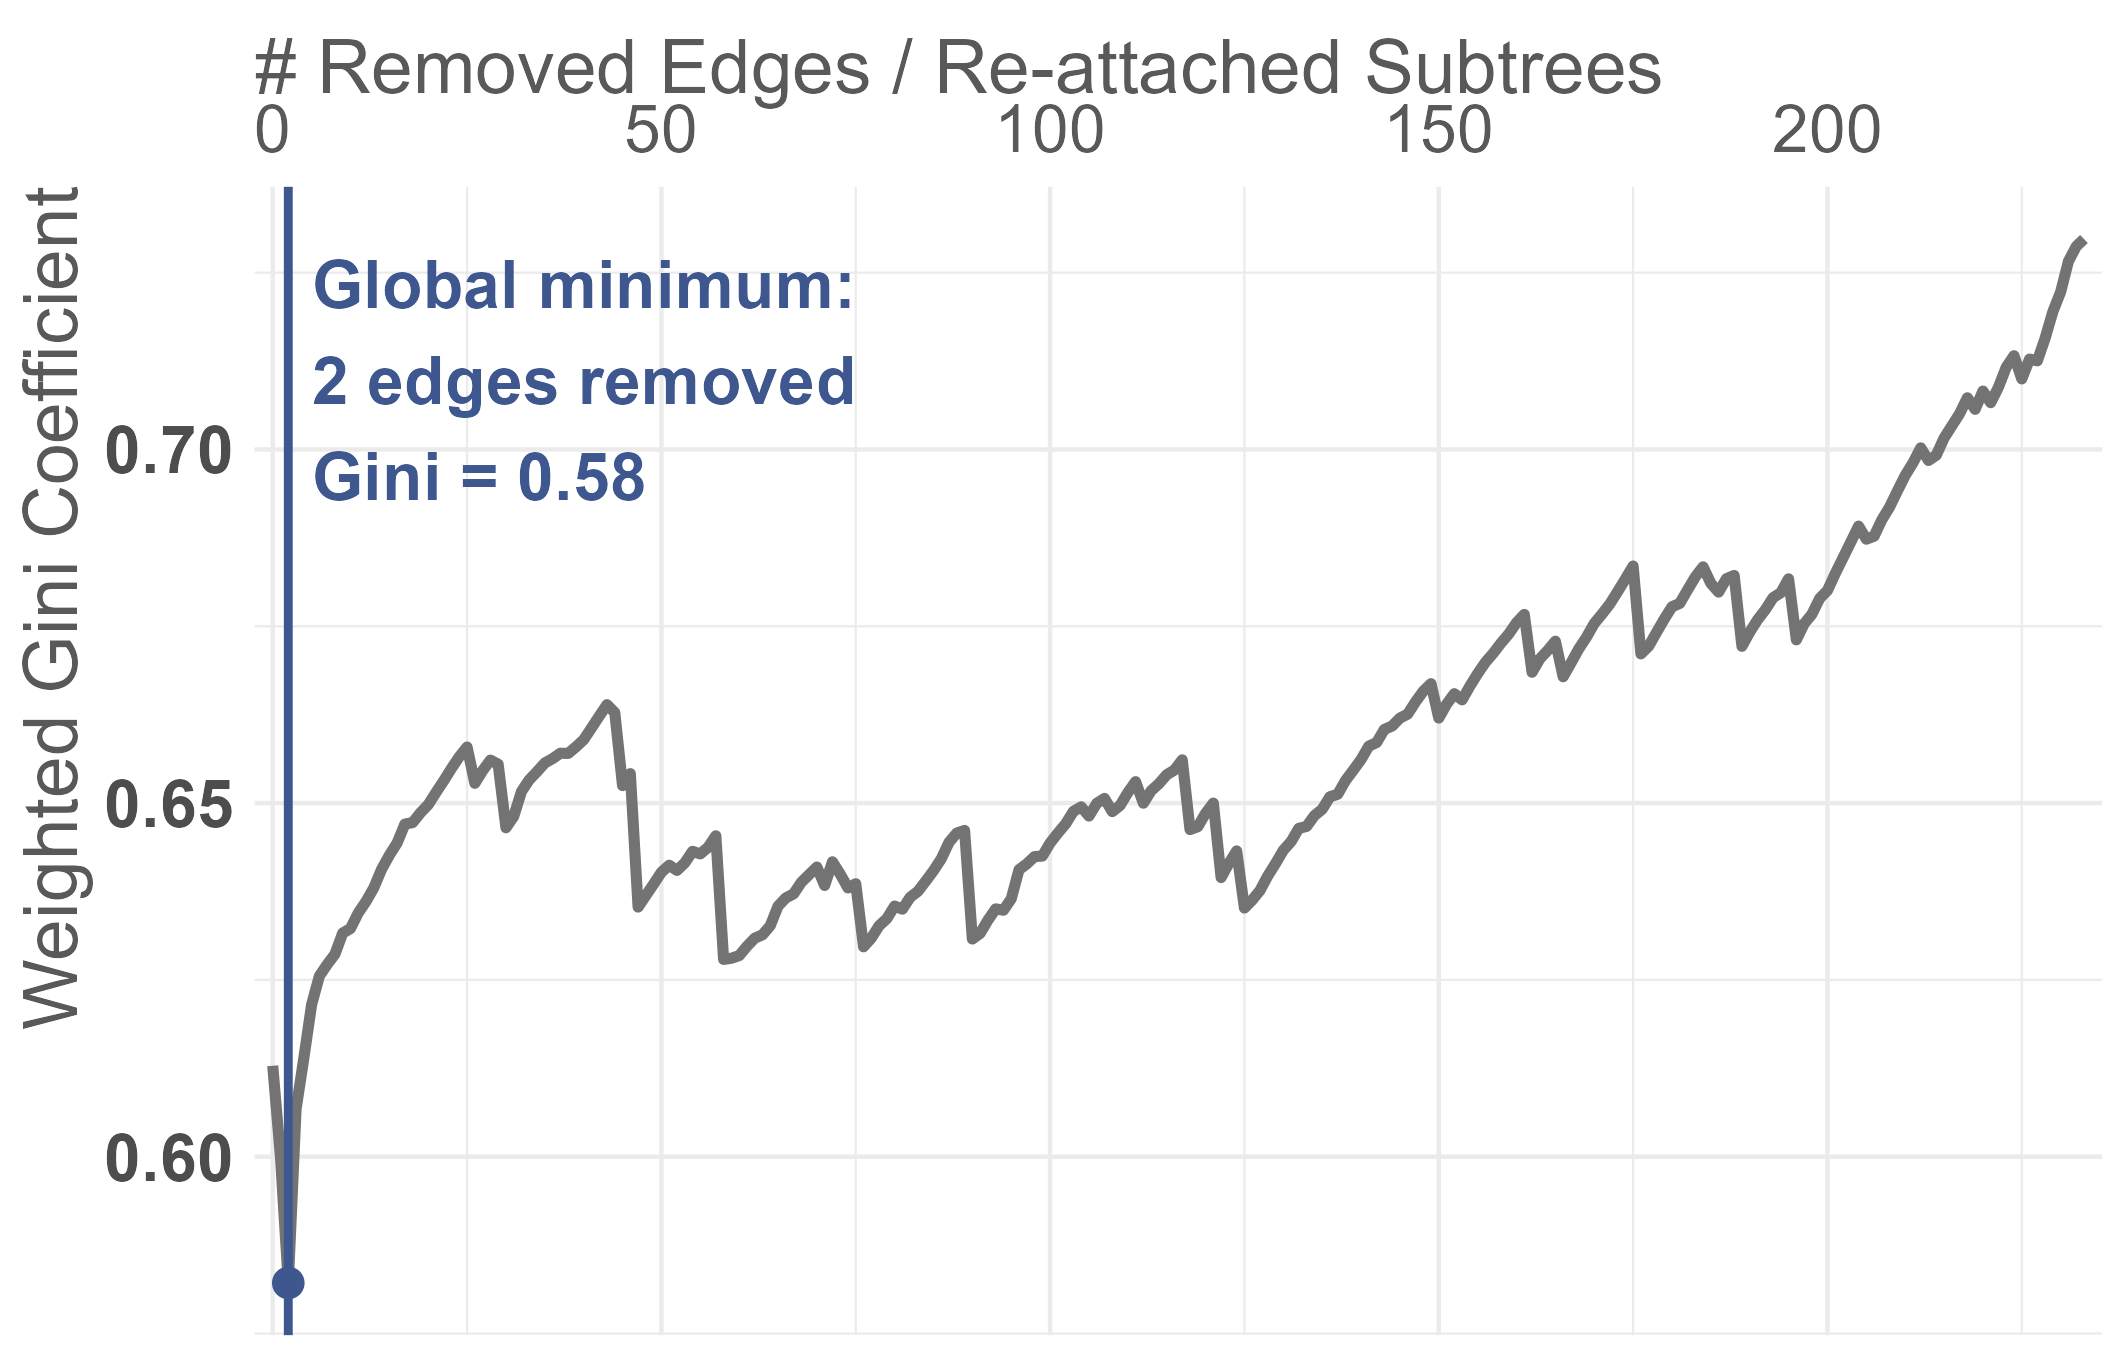
\includegraphics[width=\columnwidth]{figures/balancing_gini_trajectory.png}
  \caption{Weighted Gini coefficient (0–1) across iterations of cutting weak genre links and reconnecting dangling subtrees to \textit{POPULAR MUSIC}.}
\label{fig:rq1_gini_trajectory}
\end{figure}

\begin{table}[htpb]
\centering
\begin{tabular}{llll}
Level & \# nodes & \# tracks & Gini   \\
\hline
1 & 3        & \begin{tabular}[c]{@{}l@{}}total: 47,846 (29\%)\\12,472; 16,401; \\and 18,973\end{tabular}                & 0.136  \\
\hline
2 & 119      & \begin{tabular}[c]{@{}l@{}}total: 90,381 (54\%)\\median: 263\\IQR: 789~\\range:10.4 to 5832\end{tabular} & 0.643  \\
\hline
3 & 110      & \begin{tabular}[c]{@{}l@{}}total: 29,343 (17\%)\\median: 156\\IQR: 259~\\range:14.7 to 1496\end{tabular} & 0.531  \\
\hline
4 & 2        & \begin{tabular}[c]{@{}l@{}}total: 192 (0.1\%)~\\55.6 and 136\end{tabular}                                 & 0.420 
\end{tabular}  
\caption{Structure of COMGET-G at different hierarchy levels; track counts are sums of genre tag assignment probabilities in POPTRAG.}
\label{tab:rq1_structure}
\end{table}

The initial POPTRAG \textit{genre} co-occurrence network contained 234 \textit{genre} nodes forming a single connected component with 45.14\% density, indicating relatively high inter-tag connectivity. By median, \textit{genres} co-occurred with 97 different others (IQR 63.5; range 3 for \textit{waltz} to 229 for \textit{pop}), revealing large differences between niche and ubiquitous tags. After resolving reciprocal directions, each \textit{genre} received on average 29.5 incoming subgenre links (IQR 32; min 0; max 228 for \textit{pop rock}) and 55 outgoing supergenre links (IQR 32; min 0 for \textit{rock}; max 105 for \textit{dub}). 

The balance optimization procedure (Figure \ref{fig:rq1_gini_trajectory}) reattached \textit{pop} and \textit{hip hop} directly to \textit{POPULAR MUSIC}—\textit{pop} had formerly been subordinate to \textit{rock}, and \textit{hip hop} to \textit{pop}, however these connections where the weakest in the whole tree and their cutting resulted in clear improval of overall balance. The three weakest remaining links are \textit{electronic} to \textit{pop} (0.22), \textit{classical} to \textit{pop} (0.27), and \textit{jazz} to \textit{pop} (0.29). The final \textit{Community Music Genre Tree for popular music in Germany} (COMGET-G) is highly leaf-heavy: 89.36\% of genre-nodes lack subgenres. \textit{Rock} emerges as the largest \textit{supergenre} with 63 direct \textit{subgenres}, and only \textit{rock}, \textit{pop}, and \textit{hip hop} remain connected directly to \textit{POPULAR MUSIC}, forming three broad meta-categories. The tree exhibits four hierarchy levels (excluding the artificial root); see Table \ref{tab:rq1_structure} for structural details. An interactive visualization of COMGET-G is available in the digital appendix.


\section{RQ2: Scalable Granularity}
\subsection{Methods: Folding Algorithm (FOLDCAT)}
To derive a scalable number of broader \textit{genre categories} suitable for diverse research questions and statistical applications from COMGET-G, we developed a greedy folding algorithm (FOLDCAT) with three objectives: optimal \textit{genre category} balance, a user-selectable number of \textit{genre categories}, and sufficient track counts per \textit{genre} for robust machine learning and statistical analysis. FOLDCAT iteratively processes leaf \textit{genres} beginning with those deepest in the hierarchy and largest in track count, continuing to the root. For each leaf \textit{genre}, the algorithm checks whether it meets a minimum track count threshold. If it does and its supergenre can sustain removal, the algorithm keeps that leaf \textit{genre} as a \textit{genre category}. Otherwise, the algorithm absorbs the leaf \textit{genre}---along with its siblings and any descendants already processed---into its supergenre by remapping all track assignments upward. This procedure continues until all remaining \textit{genres} meet the minimum threshold. 

Here, \textit{genre size} is again computed as the sum of vote-weighted assignment probabilities across all tracks. For a desired number of \textit{genre categories}, users select the folding solution corresponding to a local Gini minimum, drawing on a hierarchy-level-weighted Gini coefficient (see section~\ref{sec:gini_explanation}), thereby ensuring well-balanced \textit{categories} across all hierarchy levels. A detailed flowchart of this procedure appears in the appendix. For the present exemplary analysis using the POPTRAG corpus, we conducted a grid search across minimum \textit{genre sizes} from 1,000 to 15,000 in increments of 5, then selected four different local Gini minima from the results for comparison.


\subsection{Results: Germany's Popular Music Genre Categories}

\begin{figure}[htbp]
  \centering
  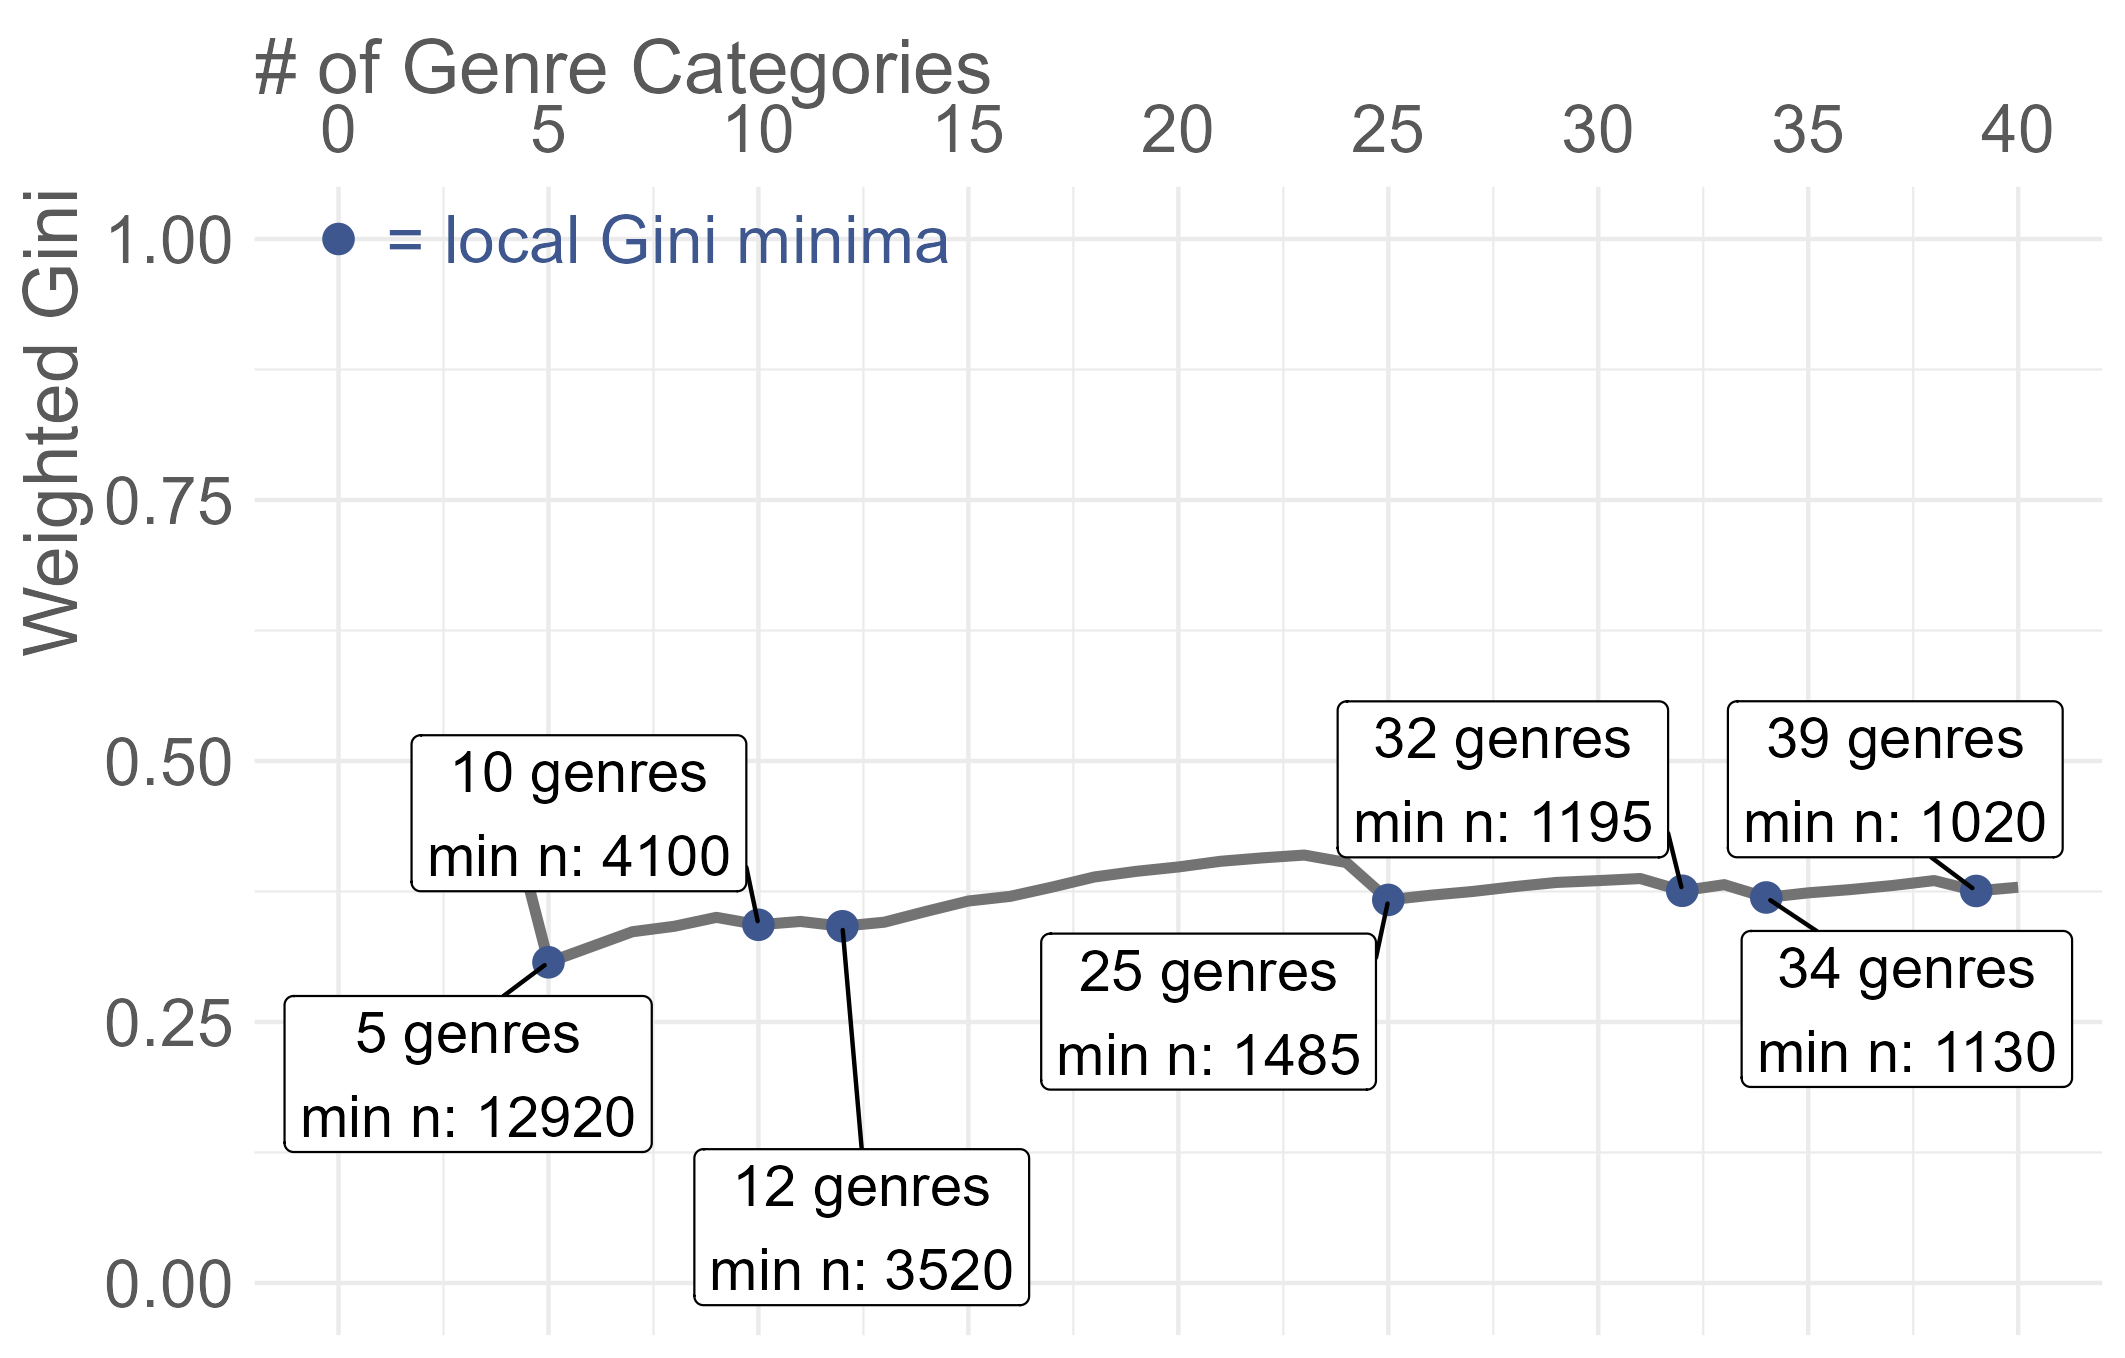
\includegraphics[width=\columnwidth]{figures/folding_gini_trajectory.png}
  \caption{Weighted Gini coefficient (0--1) across COMGET-G folding solutions for minimum track counts from 1,000 to 15,000 in increments of 5, using the POPTRAG corpus.}
\label{fig:rq2_gini_trajectory}
\end{figure}

For our POPTRAG corpus, the folding algorithm identified multiple optimal solutions for a COMGET-G (Figure~\ref{fig:rq2_gini_trajectory}): a low-granularity solution with 5 \textit{genre categories} (min. 12,930 tracks, Gini 0.307), medium-granularity solutions with 10 and 12 \textit{genre categories} (min. 4,100 and 3,520 tracks; Gini 0.343 and 0.342), a high-granularity solution with 25 \textit{genre categories} (min. 1,485 tracks, Gini 0.367), and solutions with higher granularity, comprising 32, 34, and 38 \textit{genre categories} (min. 1,195, 1,130, 1,020 tracks; Gini 0.376, 0.369, 0.375). We focused subsequent analyses on solutions with 5, 12, 25, and 32 \textit{genre categories}, representing different granularities suitable for various research questions (Figure~\ref{fig:rq2_tree}).


\begin{figure}[htbp]
  \centering
  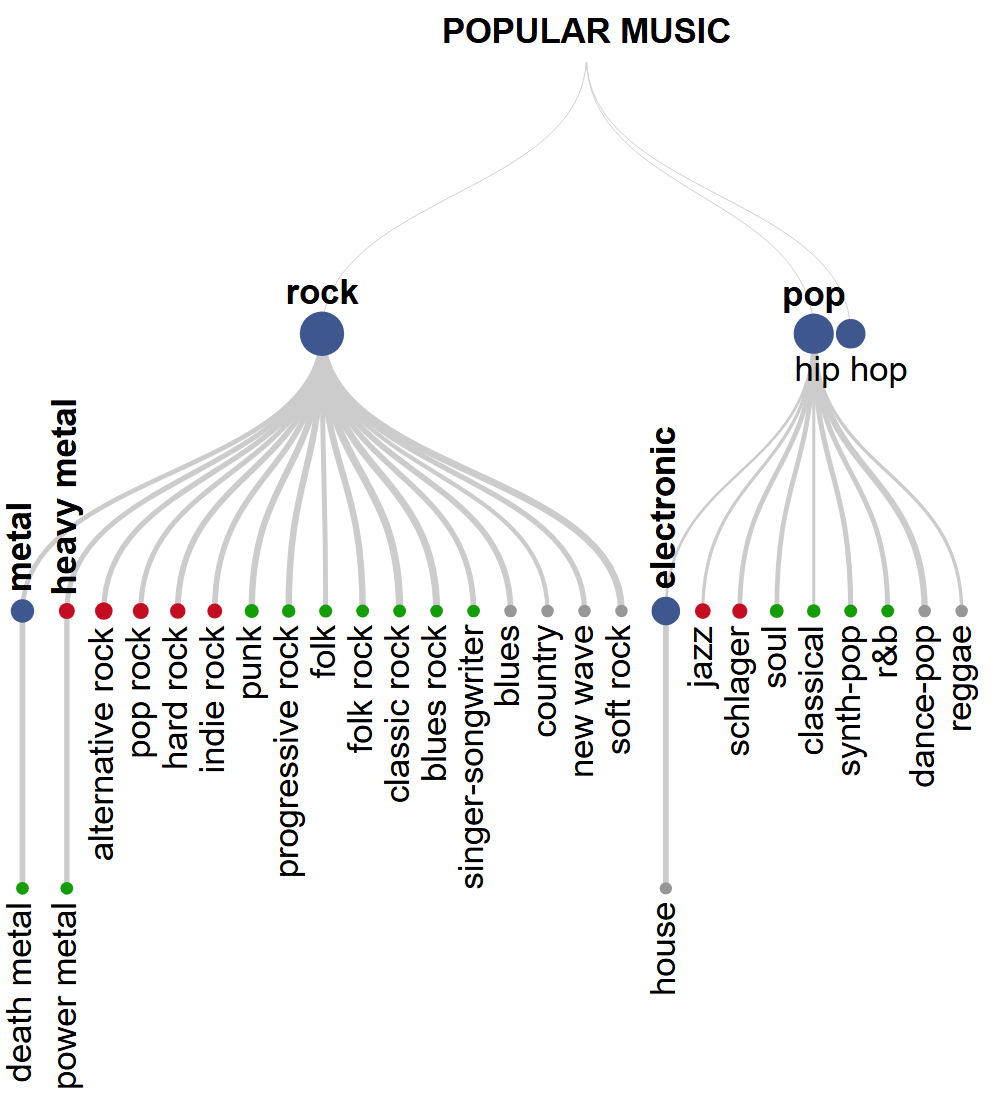
\includegraphics[width=\columnwidth]{figures/supergenre_hierarchy.png}
  \caption{Folded COMGET-G hierarchies for POPTRAG corpus at four different granularities (5, 12, 25, 32 \textit{genre categories}). Colors indicate additional categories introduced at each finer levels of granularity (blue = 5; red = 12; green = 25; grey = 32). Node size represents approximate track count in POPTRAG (sum of vote-weighted assignment probabilities).}
\label{fig:rq2_tree}
\end{figure}

COMGET-G5 comprises \textit{rock}, \textit{pop}, \textit{hip hop}, \textit{electronic}, and \textit{metal} (in descending order of track count). In COMGET-G12, \textit{jazz} and \textit{schlager} emerge as further distinct \textit{pop subgenre categories}, while \textit{rock subgenre categories} including \textit{heavy metal}, \textit{alternative rock}, \textit{pop rock}, \textit{hard rock}, and \textit{indie rock} appear at the same level. Notably, listeners do not classify \textit{heavy metal} as a \textit{subgenre category} of \textit{metal} but as a direct \textit{subgenre category} of \textit{rock} on the same hierarchy level as \textit{metal}.

COMGET-G25 introduces further \textit{rock subgenre categories} (\textit{punk}, \textit{progressive rock}, \textit{folk}, \textit{folk rock}, \textit{classic rock}, \textit{blues rock}, \textit{singer-songwriter}) and additional \textit{pop subgenre categories} (\textit{soul}, \textit{classical}, \textit{synth-pop}, \textit{r\&b}). A third hierarchy level appears with \textit{death metal} as a \textit{subgenre category} of \textit{metal} and \textit{power metal} as a \textit{subgenre category} of \textit{heavy metal}. COMGET-G32 adds \textit{house} as an \textit{electronic subgenre category} and additional \textit{rock} and \textit{pop} branches (\textit{blues}, \textit{country}, \textit{new wave}, \textit{soft rock}, \textit{dance-pop}, \textit{reggae}). \textit{hip hop} \textit{subgenre categories} appear only in more fine-grained solutions (\textit{pop rap} as 33rd genre, \textit{trap} as 38th genre).


\section{RQ3: Validity and ML-Classifier}
\subsection{Methods: Single Labels, Content Validity, Features, Workflow}
To compare the COMGET-G genre assignments to other folksonomies and for training a classifier, each track in the corpus obtained a \textit{single COMGET-G genre label} via majority voting: all valid original \textit{MusicBrainz} tags assigned to a track were mapped to their \textit{category assignment} in folded COMGET-G, then each track received the \textit{category} tag with the highest summed votes. Ties were resolved by selecting the \textit{genre category} with lower total assignment probability in the full dataset, thereby favoring more detailed \textit{genre category} assignments. We derived \textit{single genre labels} for each track at four levels of granularity (COMGET-G5, COMGET-G12, COMGET-G25, COMGET-G32). For demonstrating the content validity of our exemplary 12-genre solution, we compared resulting \textit{genre category assignments} to the genre labels assigned by the \textit{Discogs} community using a contingency table. 

To determine if an automated classifier could predict the COMGET-G \textit{genre categories} identified by FOLDCAT, we trained independent classifiers for each. To that end, we augmented POPTRAG with 192 descriptor variables covering \textit{musical style}, \textit{release context}, \textit{lyrical content}, and \textit{popularity} from music platforms \textit{Spotify}, \textit{MusicBrainz}, \textit{AcousticBrainz}, \textit{Genius}, and \textit{Deezer} via ISRC matching or fuzzy string matching via either API-access or web scraping. \textit{AcousticBrainz} provided community-calculated \textit{audio features}; \textit{MusicBrainz} supplied artist demographics (\textit{persona}, \textit{origin}, \textit{birth year}, \textit{gender}); \textit{Spotify} and \textit{Deezer} contributed \textit{popularity} metrics and \textit{Echo-Nest audio features}. From \textit{Spotify's artist-level genre} tags we derived 69 \textit{distribution-genre} flags (e.g., whether a track's artist is tagged as `reggae' on \textit{Spotify}) by applying the same co-occurrence algorithm used to build COMGET-G but operating on Spotify artist genres. \textit{Spotify's distribution genre} categories can be a valuable signal of release milieu and test whether industry framing influences how listeners ultimately categorize music.

In our workflow, we first discarded observations with more than 40\% missing values on any variable, retaining 155,093 tracks (92\%). We then performed an 80/20 train–holdout split at the artist level to mitigate artist leakage effects~\citep{flexerEffectsAlbumArtist2010}. For training, we employed 5-fold cross-validation (also group-split by artist) for hyperparameter tuning. To stabilize categorical predictors, we drew a 20\% subsample of the training set, created artist‑grouped CV folds on that subsample, and relabeled any factor level that occurred fewer than 100 times in at least one fold as ``other''. Predictors that collapsed to a single ``other''-level as well as two‑level predictors where the ``other'' level had fewer than 100 observations, were removed. This cleaning reduced the number of variables from 192 to 149. All remaining categorical predictors were dummy-coded, using the most common level as the reference.

Preprocessing was applied in sequence within each single fold: median imputation, adaptive class balancing (excluded fors holdout set), and normalization. Adaptive balancing used a single tunable \textit{target-ratio} parameter governing rebalancing degree. The algorithm computed a reference count from outcome class frequencies (median for $\leq$ 10 classes; 60th percentile for 11–20 classes; 65th percentile for $>$ 20 classes), then downsampled classes exceeding reference $\times$ \textit{target ratio} using NearMiss~\citep{zhangKNNApproachUnbalanced2003} and upsampled classes below reference $\div$ \textit{target ratio} using Borderline SMOTE~\citep{hanBorderlineSMOTENewOverSampling2005} or regular SMOTE when sufficient danger observations were unavailable. This approach preserved more data than fixed-ratio sampling while remaining tunable: \textit{target ratio} = 1 enforced perfect balance; higher values retained original imbalance. The reference-count heuristic scaled to problem complexity, preventing excessive downsampling at higher resolutions.

For hyperparameter search, we employed Bayesian optimization~\citep{snoekPracticalBayesianOptimization2012a} with a Latin hypercube initial grid ~\citep{husslageSpacefillingLatinHypercube2011}, early stopping if no improvement occurred after 10 iterations, and exploration of uncertain hyperparameter regions after 5 iterations without improvement. The best hyperparameters were selected using the one-standard-error rule~\citep{hastieModelAssessmentSelection2009}. We tuned hyperparameters across five folds using the macro-averaged F1 score (mean per-class F1, set to 0 for unpredicted classes) to treat all \textit{genres} equally during evaluation. 

Initially, we evaluated four different supervised ML algorithms based on a 20\% subsample of the training data at low and medium granularity to identify the most suitable learner: elastic net (GLMNET; Tay et al.,~\citeyear{tayetalElasticNet2023}), regularized discriminant analysis (RDA; Weihs et al.,~\citeyear{weihsetalKlaR2005}), random forest (RF; Wright and Ziegler,~\citeyear{wrightetalRanger2017}), and light gradient boosted machine (LightGBM; Shi et al.,~\citeyear{shietalLightgbm2025}). For each we tuned key hyperparameters: GLMNET — \textit{penalty} and \textit{mixture} in [0, 1]; RDA — \textit{covariance fraction} and \textit{identity fraction} in [0, 1]; RF — \textit{feature fraction considered at each split} in [1, \# of predictors] and \textit{leaf node size} in [1, 100]; number of trees was set to 500 for tuning and 1000 for final models; LightGBM — \textit{boosting rounds} in [50, 2000], \textit{learning rate} in [0.001, 0.1], \textit{leaf node size} in [1, 100], \textit{tree depth} in [3, 15], and \textit{feature fraction} in [1, \# of predictors]. For all learners, the target ratio used for adaptive balancing was tuned in [1, max(obsevations per class)/min(observations per class)]. For choosing the best learner, we employed a coarse hyperparameter search with a 10-level initial grid and a maximum of 25 iterations for Bayesian optimization.

After selecting the learner with best performance accross folds, we performed a more extensive hyperparameter search with a 20-level initial grid and a maximum of 50 iterations with 5-fold crossvalidation on the full training set for all levels of granularity, trained the final classifiers on the full training set, and evaluated results on the holdout set. \textit{Community certainty} served as a reference point for evaluating final classifier performance, since ML models cannot exceed the consistency of the underlying human community assignments. For this comparison \textit{certainty} was computed as the mean assignment probability across votes for each track assigned to the \textit{single-label genre}. All random operations used the seed 42 for reproducibility.


\subsection{Results: Comparison against \textit{Discogs} taxonomy}
\begin{figure}[htbp]
  \centering
  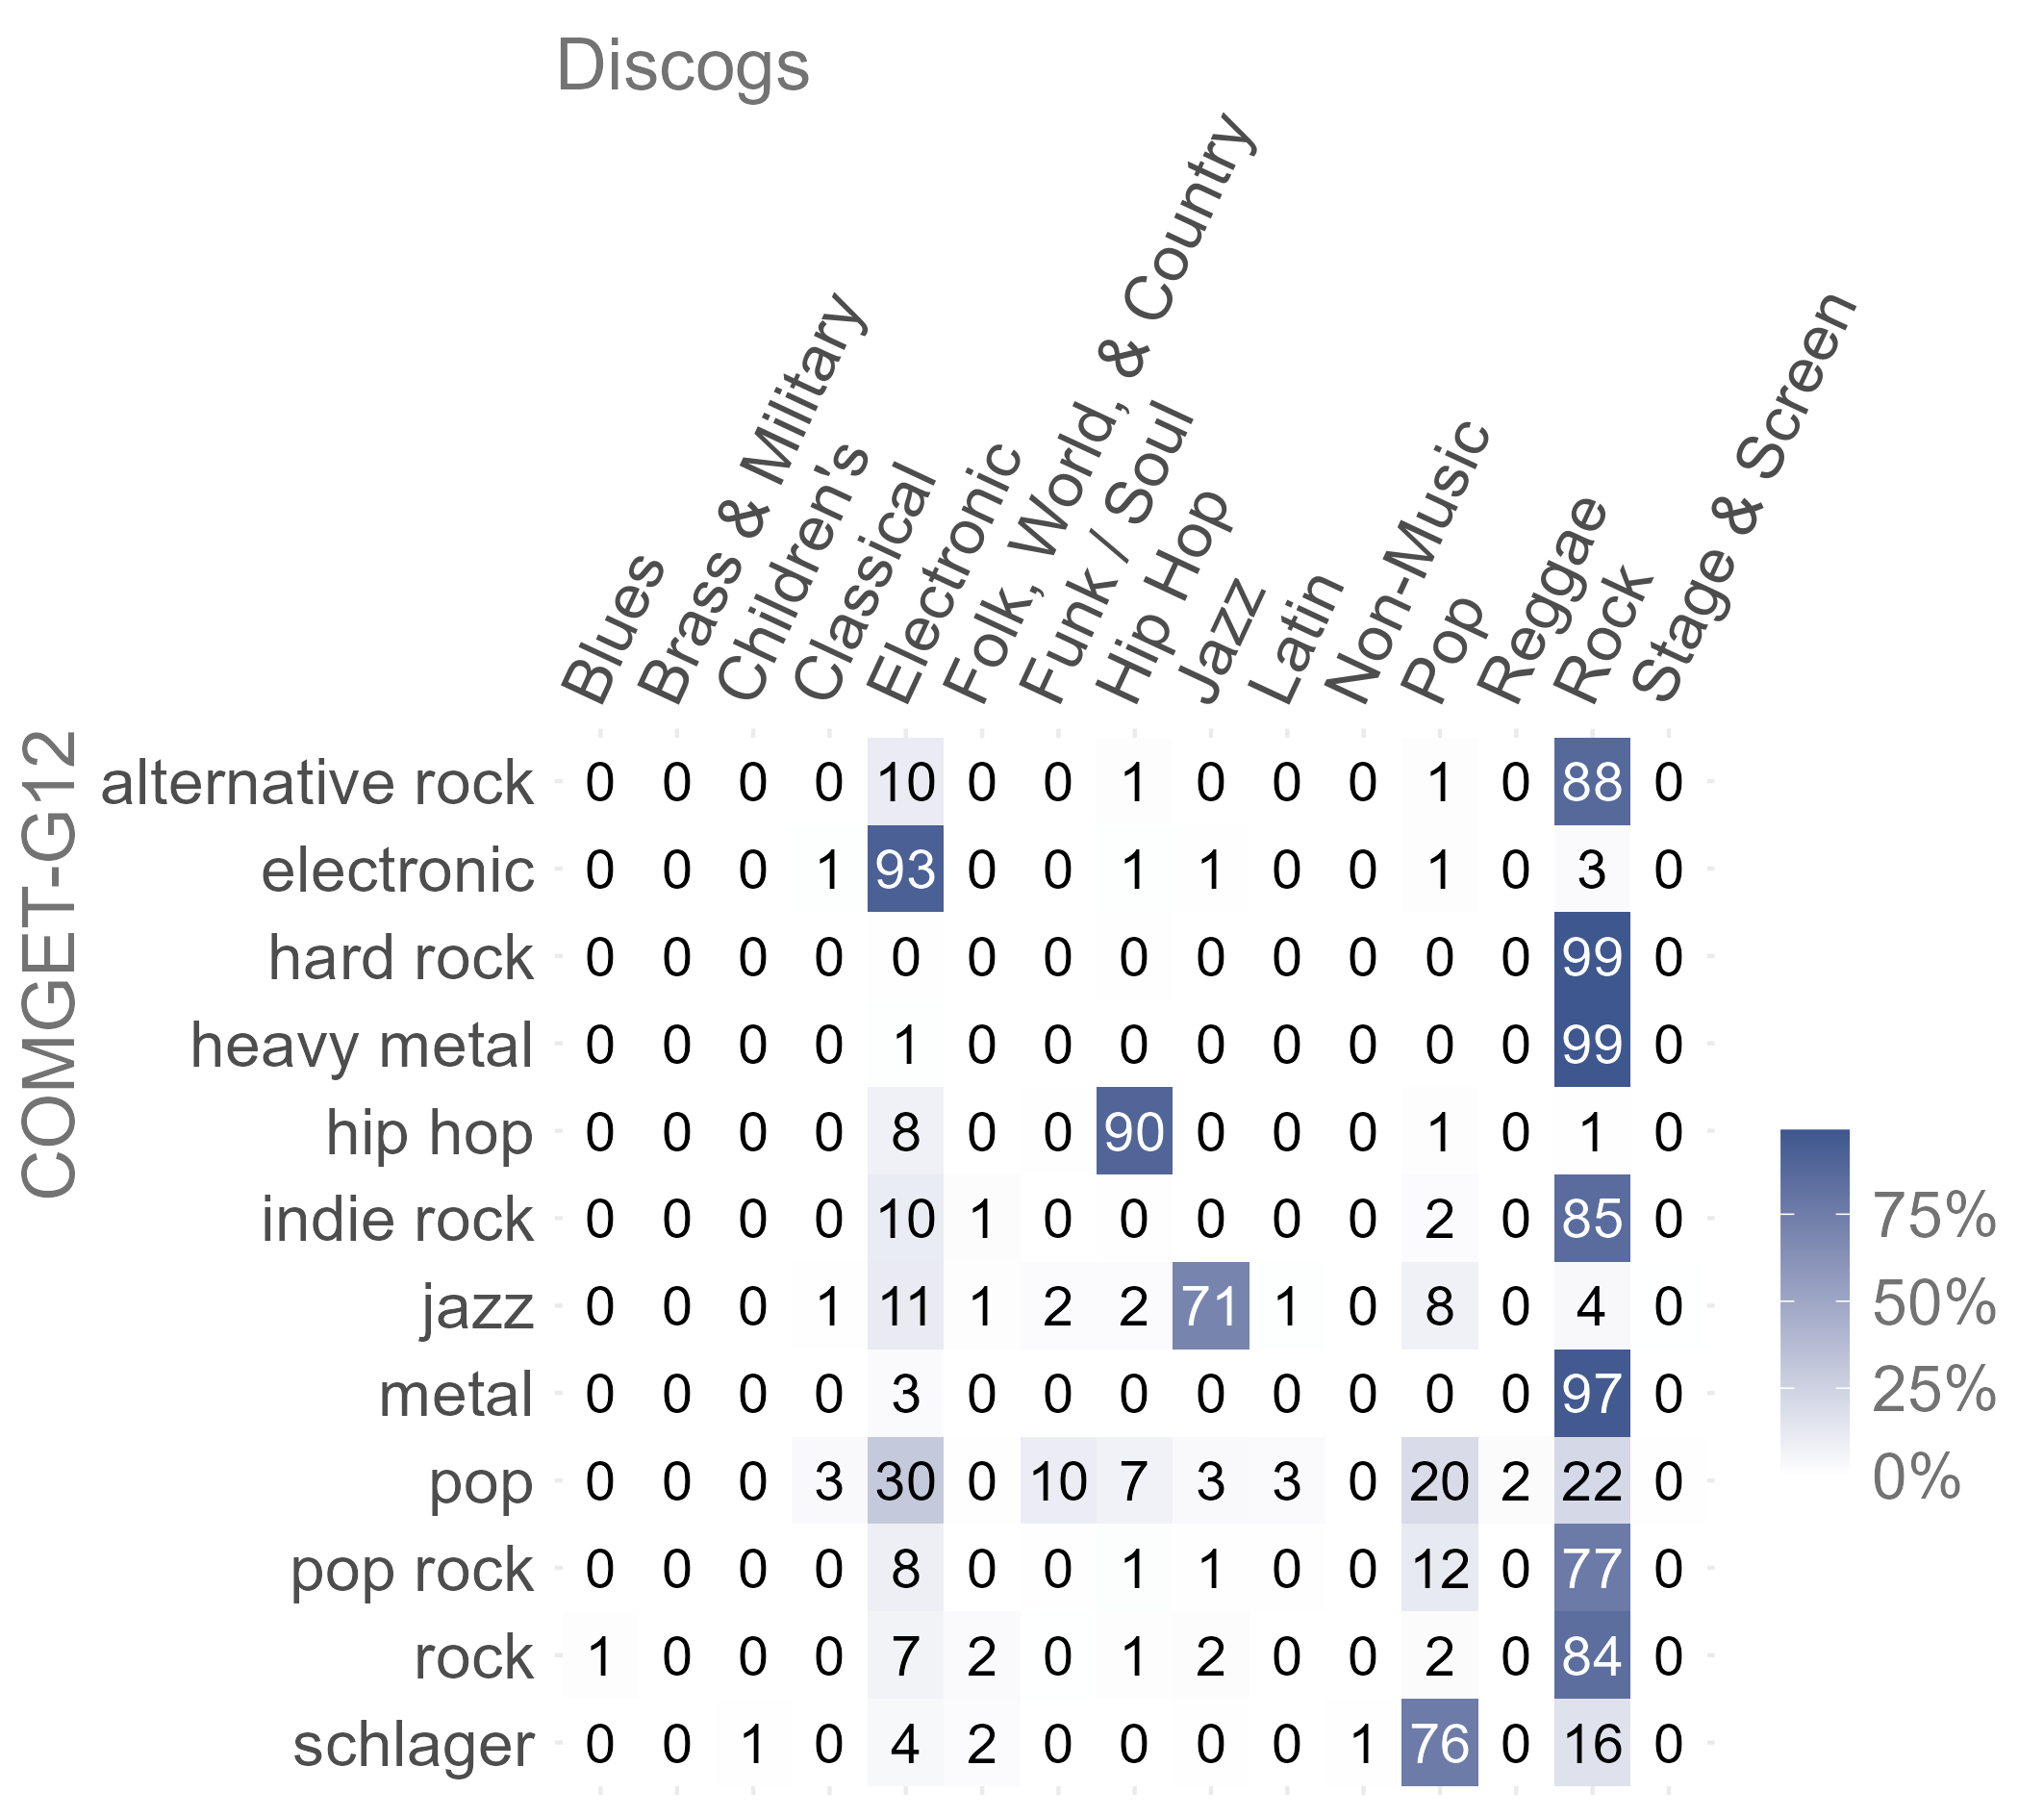
\includegraphics[width=\columnwidth]{figures/dc_contingency.png}
  \caption{Contingency table comparing COMGET-G12 and \textit{Discogs} genre assignments; values show $P(\text{Discogs} \mid \text{COMGET-G12})$.}
  \label{fig:rq2_dc}
\end{figure}

\textit{Discogs'} 15-genre taxonomy approximates COMGET-G12 in scale. For approximately 5\% of tracks with COMGET-G assignments, we found no \textit{Discogs} counterpart, introducing minimal popularity bias. The contingency table (Figure~\ref{fig:rq2_dc}) reveals strong alignment for \textit{electronic}, \textit{hard rock}, and \textit{metal}. Even where \textit{Discogs} includes a \textit{Jazz} category, COMGET-G's \textit{jazz} overlaps substantially with \textit{Discogs'} \textit{Electronic} and \textit{Pop}. Similarly, \textit{pop rock} is distributed across Discogs' \textit{Rock}, \textit{Pop}, and \textit{Electronic}; \textit{schlager} emerges in \textit{Pop} (similar label to its COMGET-G \textit{supergenre}) with minor overlap to \textit{Rock}. Five \textit{Discogs} categories—\textit{Blues}, \textit{Brass \& Military}, \textit{Children's}, \textit{Non-music}, and \textit{Stage \& Screen}—show minimal correspondence to any COMGET-G12 \textit{genre category}, mostly consistent with our noise-reduction filtering and focus on popular music. COMGET-G's \textit{pop} category is distributed widely across \textit{Discogs genres} (\textit{eEectronic}, \textit{Pop}, \textit{Rock}), reflecting pop's eclectic character. Seven of twelve COMGET-G12 \textit{genre categories} overlap most strongly with \textit{Discogs' Rock}, suggesting \textit{Discogs} lacks granular rock subgenre category labels needed to represent German popular music adequately.

\subsection{Results: Classification Performance for different degrees of granularity}
\begin{figure}[htbp]
  \centering
  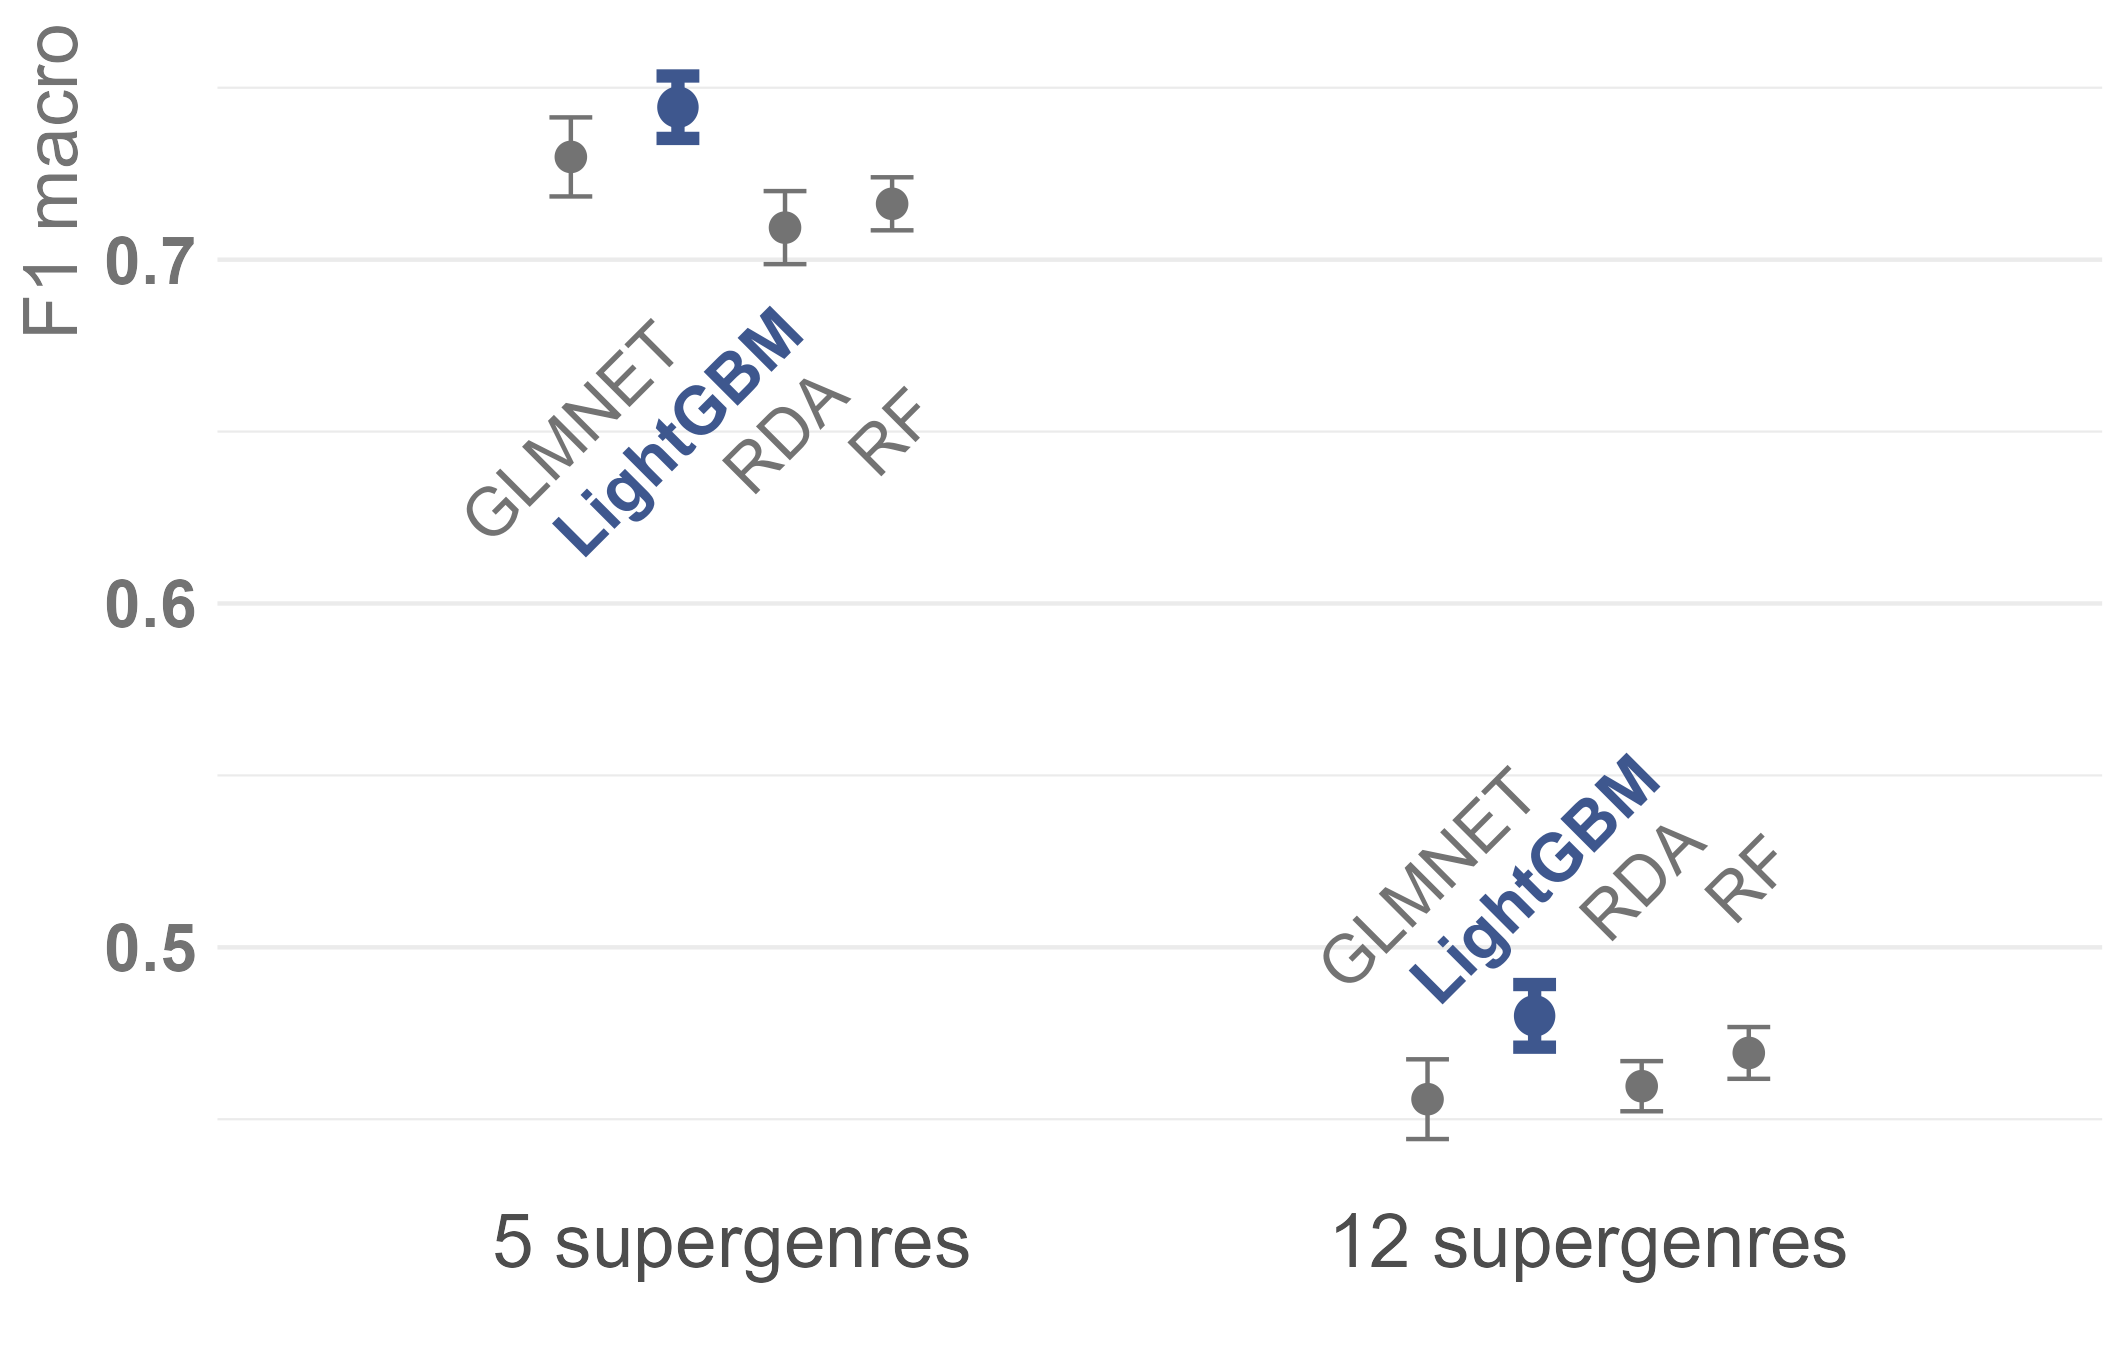
\includegraphics[width=\columnwidth]{figures/learner_comparison.png}
  \caption{Performance comparison of different learners (GLMNET, RDA, RF, GBM) on 20\% of the data set for low and medium \textit{genre} granularity; plots show mean and standard error of $\text{F1}_{\text{macro}}$ across CV folds.}
\label{fig:rq3_proto}
\end{figure}

Model comparison (Figure~\ref{fig:rq3_proto}) shows that all four learners perform similarly on the 20\% subsample in terms of macro F1. LightGBM emerged as the strongest performer at both granularities (COMGET-G5 and COMGET-G12) and was selected as the final learner for all subsequent analyses. GLMNET ranked second for COMGET-G5 but performed worst for COMGET-G12, indicating that its linear decision boundary assumption does not scale to higher-resolution classification tasks.

\begin{figure*}[htbp]
  \centering
  \begin{subfigure}[b]{\textwidth}
    \centering
    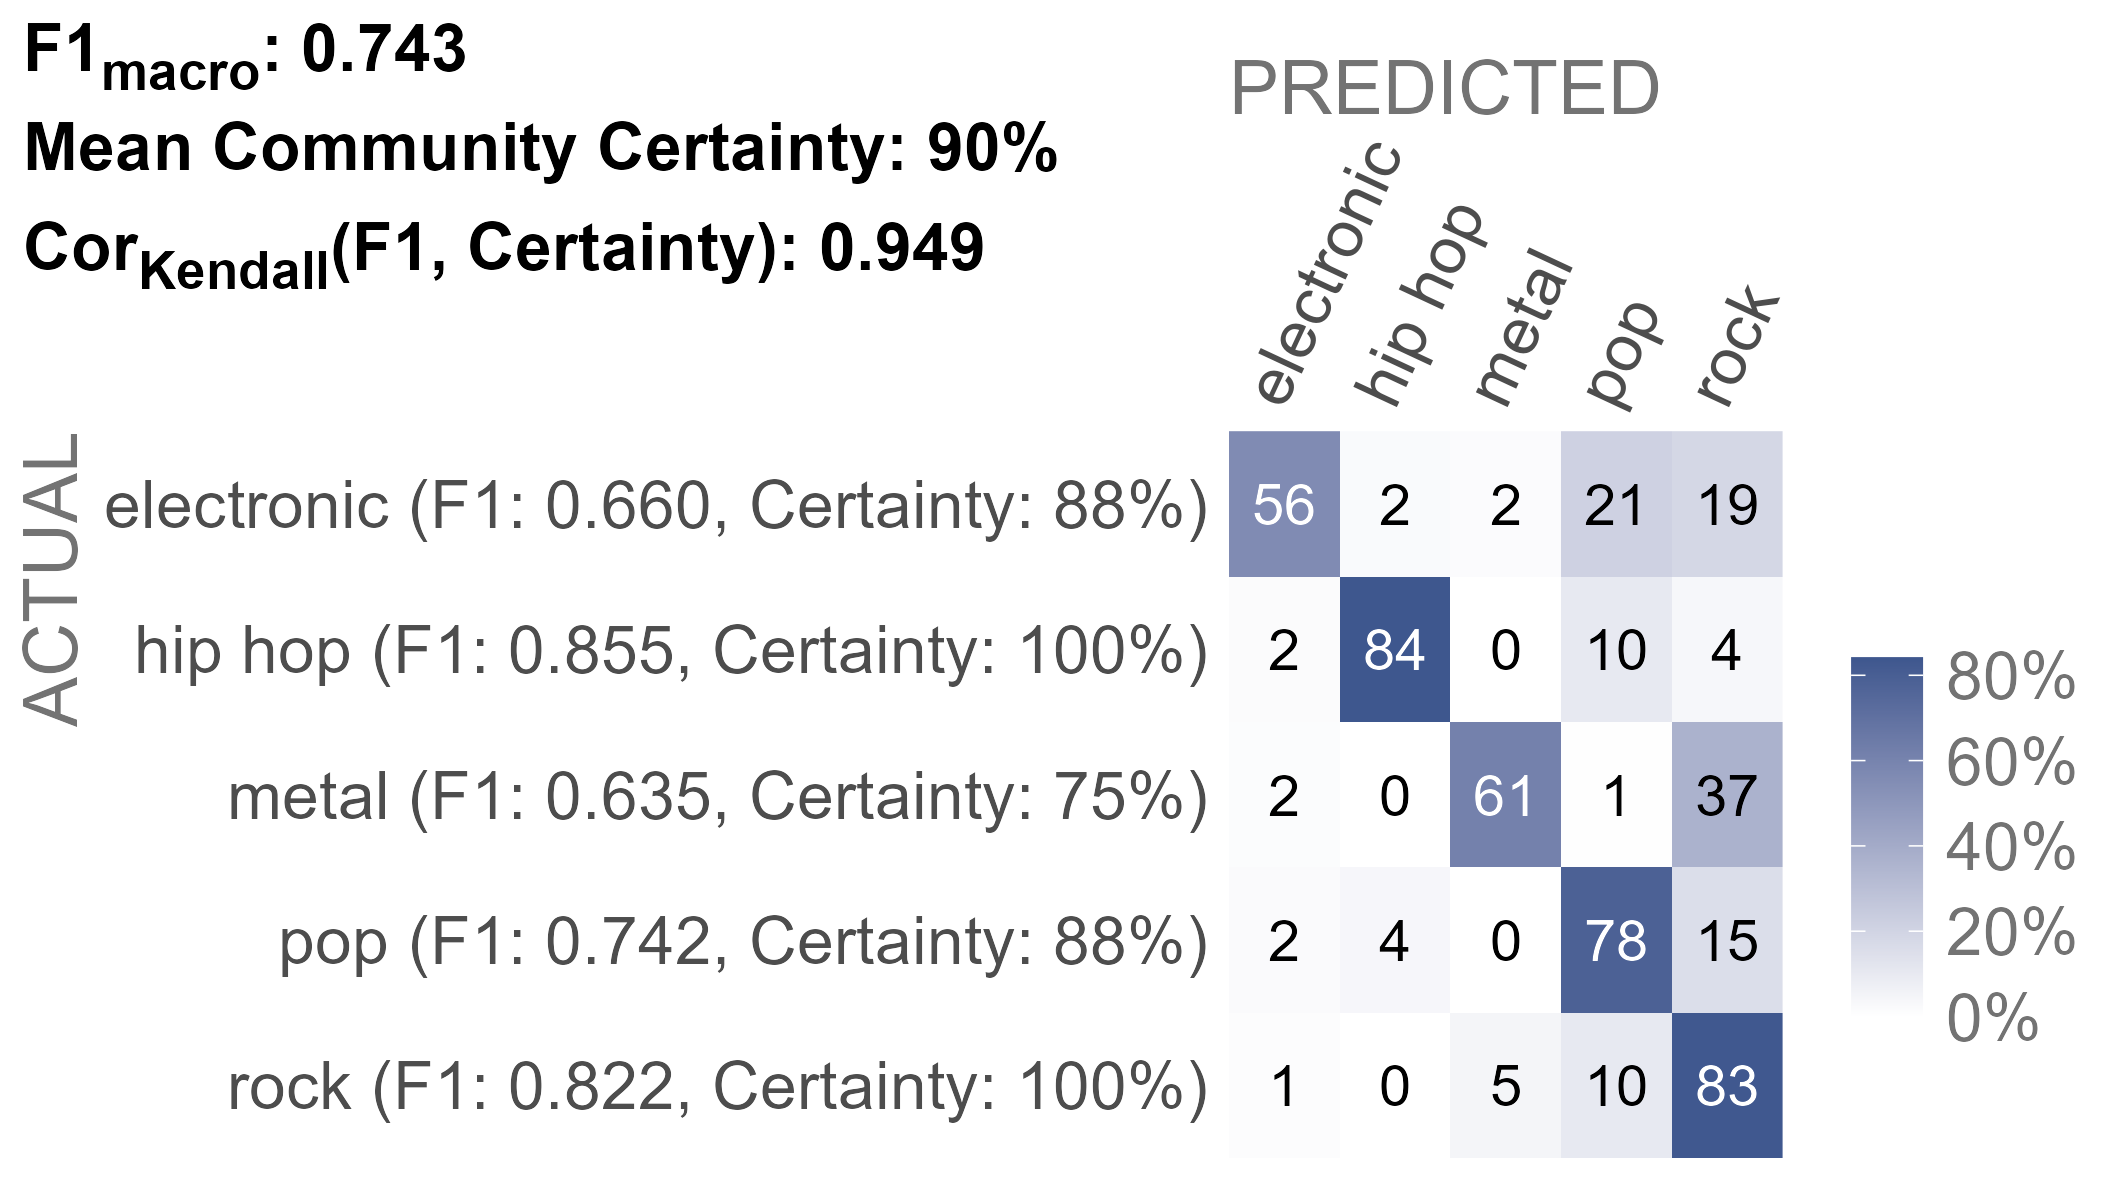
\includegraphics[width=0.57\linewidth]{figures/lightgbm_lowres_cm.png}
    \caption{COMGET-G5}
    \label{fig:rq3_cm_low}
  \end{subfigure}
  \hfill
  \vspace{1.5 cm}
  \begin{subfigure}[b]{\textwidth}
    \centering
    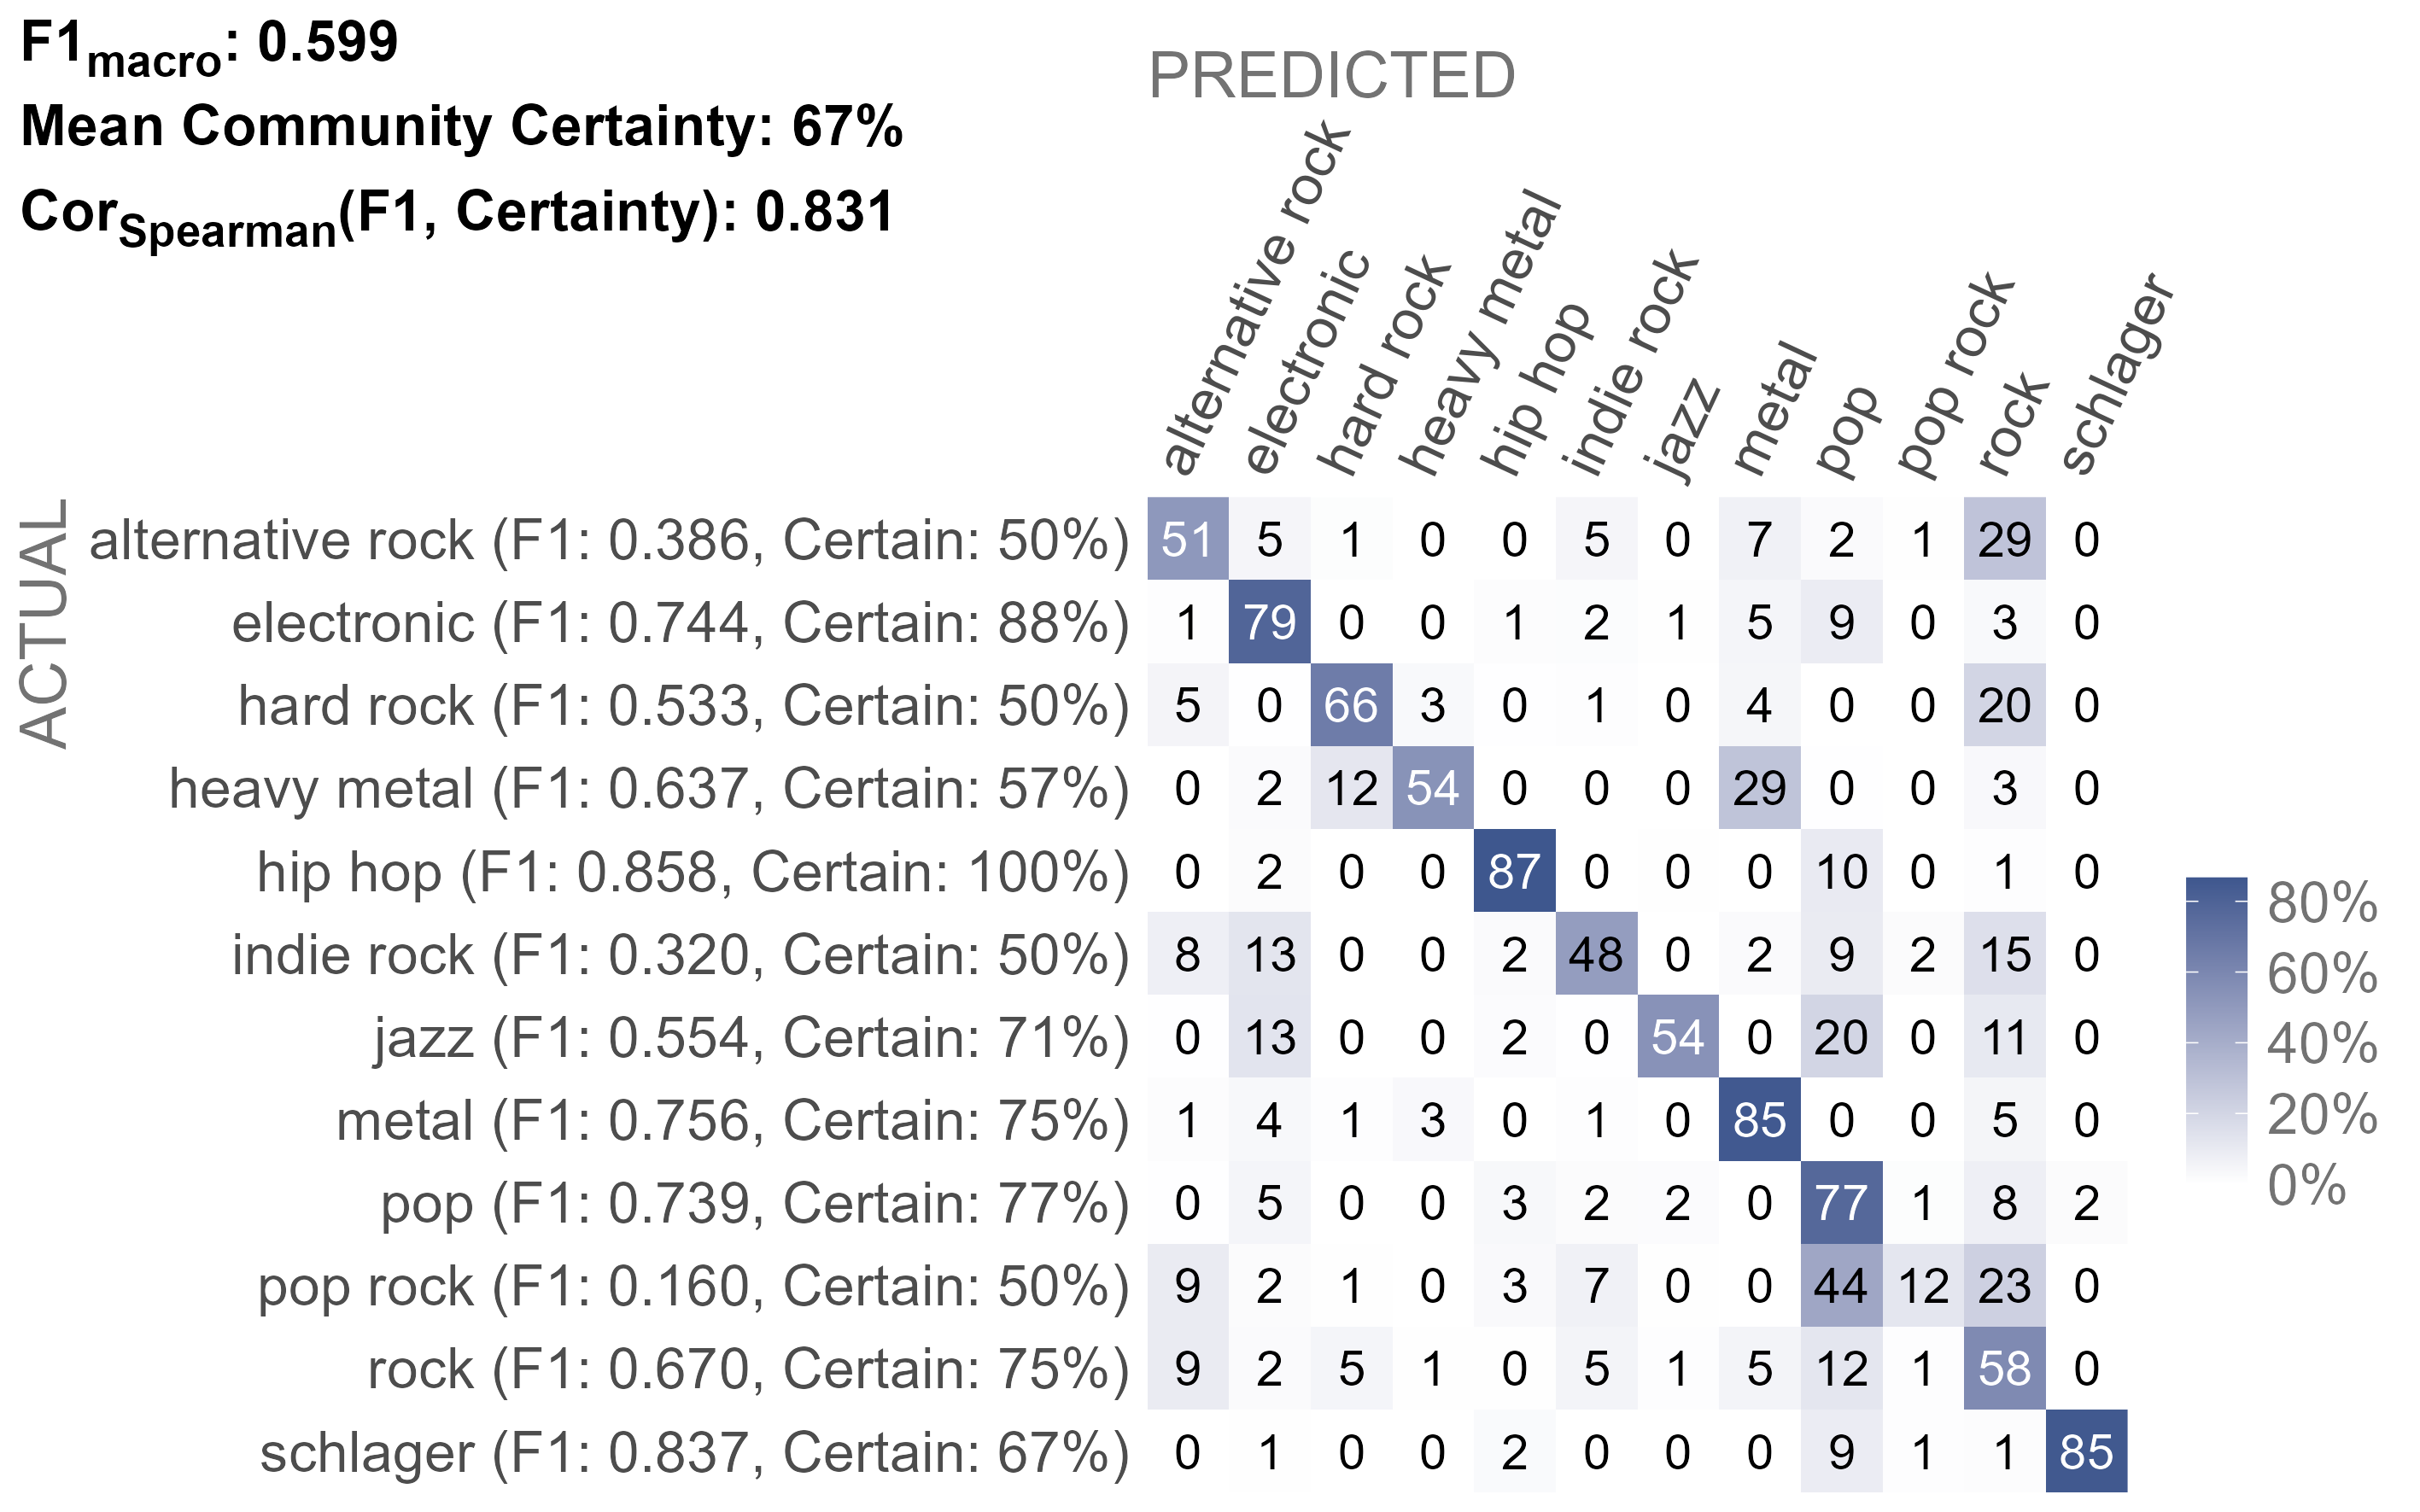
\includegraphics[width=0.8\linewidth]{figures/lightgbm_mediumres_cm.png}
    \caption{COMGET-G12}
    \label{fig:rq3_cm_medium}
  \end{subfigure}
  \caption{Confusion matrices for the final GBM models on the hold-out set. Values show $P(\text{Predicted}|\text{Actual})$; \textit{certainty} indicates the mean assignment probability for each \textit{genre category} across community votes.}
\label{fig:rq3_cm_low_medium}
\end{figure*}


\begin{table*}[htbp]
\centering
\begin{tabular}{lllllll}
\# genres & boosting rounds & tree depth & feature fraction & leaf count & learning rate & target ratio \\
\hline
5 & 854 & 4 & 83 & 98 & 0.049 & 1.177 \\
12 & 846 & 10 & 35 & 4 & 0.037 & 1.106\\
25 & 898 & 5 & 48 & 67 & 0.006 & 2.394\\
32 & 854 & 4 & 83 & 98 & 0.049 & 2.462       
\end{tabular}
\caption{Hyperparameter settings for final LightGBM models at different granularity levels.}
\label{tab:rq3_hyperparams}
\end{table*}

The final GBM models on the full dataset (Table~\ref{tab:rq3_hyperparams}) achieved $\text{F1}_{\text{macro}} = 0.803$ (SE: 0.008) on CV folds and 0.788 on the hold-out set for COMGET-G5, indicating slight overfitting. Per-class F1 correlates strongly with \textit{community assignment certainty} ($\text{Cor}_{\text{Kendall}} = 0.949$). Given mean \textit{community certainty} of 90\%, the classifier performs satisfactorily. Cohen's $\kappa = 0.723$ on the hold-out set ($\kappa_{\text{CV}} = 0.734 \pm 0.009$) meets established inter-rater agreement standards in the social sciences~\citep[p. 327]{hildebrandtInhaltsanalyse2015}.The confusion matrix (Figure~\ref{fig:rq3_cm_low}) reveals the model struggles most with \textit{electronic}, often confusing it with \textit{pop} and \textit{rock}. Electronic music's stylistic elements frequently appear across pop and rock subgenres, explaining the observed misclassifications. Similarly, \textit{metal} misclassifications with \textit{rock} reflect their close relationship.

COMGET-G12 performance degraded to $\text{F1}_{\text{macro; CV}} = 0.572 \pm 0.013$ and $\text{F1}_{\text{macro; hold-out}} = 0.599$ ($\kappa_{\text{CV}} = 0.618 \pm 0.010$; $\kappa_{\text{hold-out}} = 0.623$), with lower \textit{community certainty} (67\%), indicating greater difficulty for both community and classifier. Per-class F1 and \textit{certainty} remain highly correlated ($\text{Cor}_{\text{Kendall}} = 0.689$). The confusion matrix (Figure~\ref{fig:rq3_cm_medium}) shows primary confusion among \textit{rock subgenres} (\textit{alternative rock}, \textit{hard rock}, \textit{indie rock}, \textit{pop rock}). \textit{Heavy metal} is frequently confused with \textit{metal} but rarely vice versa, and sometimes with \textit{hard rock}, despite being recognized as distinct from \textit{rock}. \textit{Indie rock} and \textit{jazz} are often misclassified as \textit{electronic}; \textit{jazz} also confused with \textit{pop}. \textit{pop rock} performs worst (F1 = 0.160), matching its low \textit{community certainty} (50\%). It is primarily confused with \textit{rock} (F1 = 0.670, certainty = 75\%) and \textit{pop} (F1 = 0.739, certainty = 77\%), suggesting \textit{pop rock} shares ambiguous characteristics with both. Conversely, \textit{schlager} and \textit{hip hop} tracks are classified quite well (F1 = 0.837 and 0.858, respectively) despite differing \textit{community certainties} (67\% and 100\%), indicating these \textit{genres} possess very distinct characteristics in the feature space.

COMGET-G25 showed further loss in classification performance ($\text{F1}_{\text{macro; CV}} = 0.419 \pm 0.005$; $\text{F1}_{\text{macro; hold-out}} = 0.425$; $\kappa_{\text{CV}} = 0.486 \pm 0.010$; $\kappa_{\text{hold-out}} = 0.469$) alongside decreased \textit{community certainty} (56\%). The correlation between \textit{certainty} and F1 weakened ($\text{Cor}_{\text{Kendall}} = 0.538$), yet remained high, suggesting other factors influence performance at higher granularity. The confusion matrix (see appendix figure B.1a) again reveals persistent \textit{rock subgenre} confusion (\textit{alternative rock}, \textit{blues rock}, \textit{classic rock}, \textit{folk rock}, \textit{pop rock}) and \textit{metal}-related confusion (\textit{death metal}, \textit{folk rock}, \textit{hard rock}, \textit{heavy metal}, \textit{power metal}). A secondary confusion center emerges around \textit{pop}, which frequently misclassifies with \textit{alternative rock}, \textit{classical}, \textit{electronic}, \textit{folk rock}, \textit{pop rock}, \textit{r\&b}, \textit{singer-songwriter}, \textit{soul}, and \textit{synth-pop}. The model performs well (F1 > 0.7) on \textit{classical}, \textit{death metal}, \textit{electronic}, and \textit{hip hop}—\textit{genres} with distinct feature signatures and moderate to high \textit{community certainty} (ranging 50\%-100\%). Poor performers (\textit{alternative rock}, \textit{classic rock}, \textit{folk}, \textit{folk rock}, \textit{pop rock}, \textit{power metal} with F1 ranging 0.026-0.176, \textit{certainty} ranging 33\%-50\%) represent fuzzy \textit{genres} difficult to classify for both community and model.

Consistent with decreased community certainty (54\%), the model for COMGET-G32 showed a lower classification performance ($\text{F1}_{\text{macro; CV}} = 0.400 \pm 0.003$; $\text{F1}_{\text{macro; hold-out}} = 0.403$; $\kappa_{\text{CV}} = 0.477 \pm 0.005$; $\kappa_{\text{hold-out}} = 0.486$, see appendix figure B.1b) . Importantly, the correlation between \textit{certainty} and F1 recovered notably ($\text{Cor}_{\text{Kendall}} = 0.643$), indicating \textit{community uncertainty} becomes the dominant performance factor at extreme granularity. Given similarity to COMGET-G25, detailed confusion matrix results appear in the digital appendix.


\begin{figure}[htbp]
  \centering
  \begin{subfigure}[b]{\columnwidth}
    \centering
    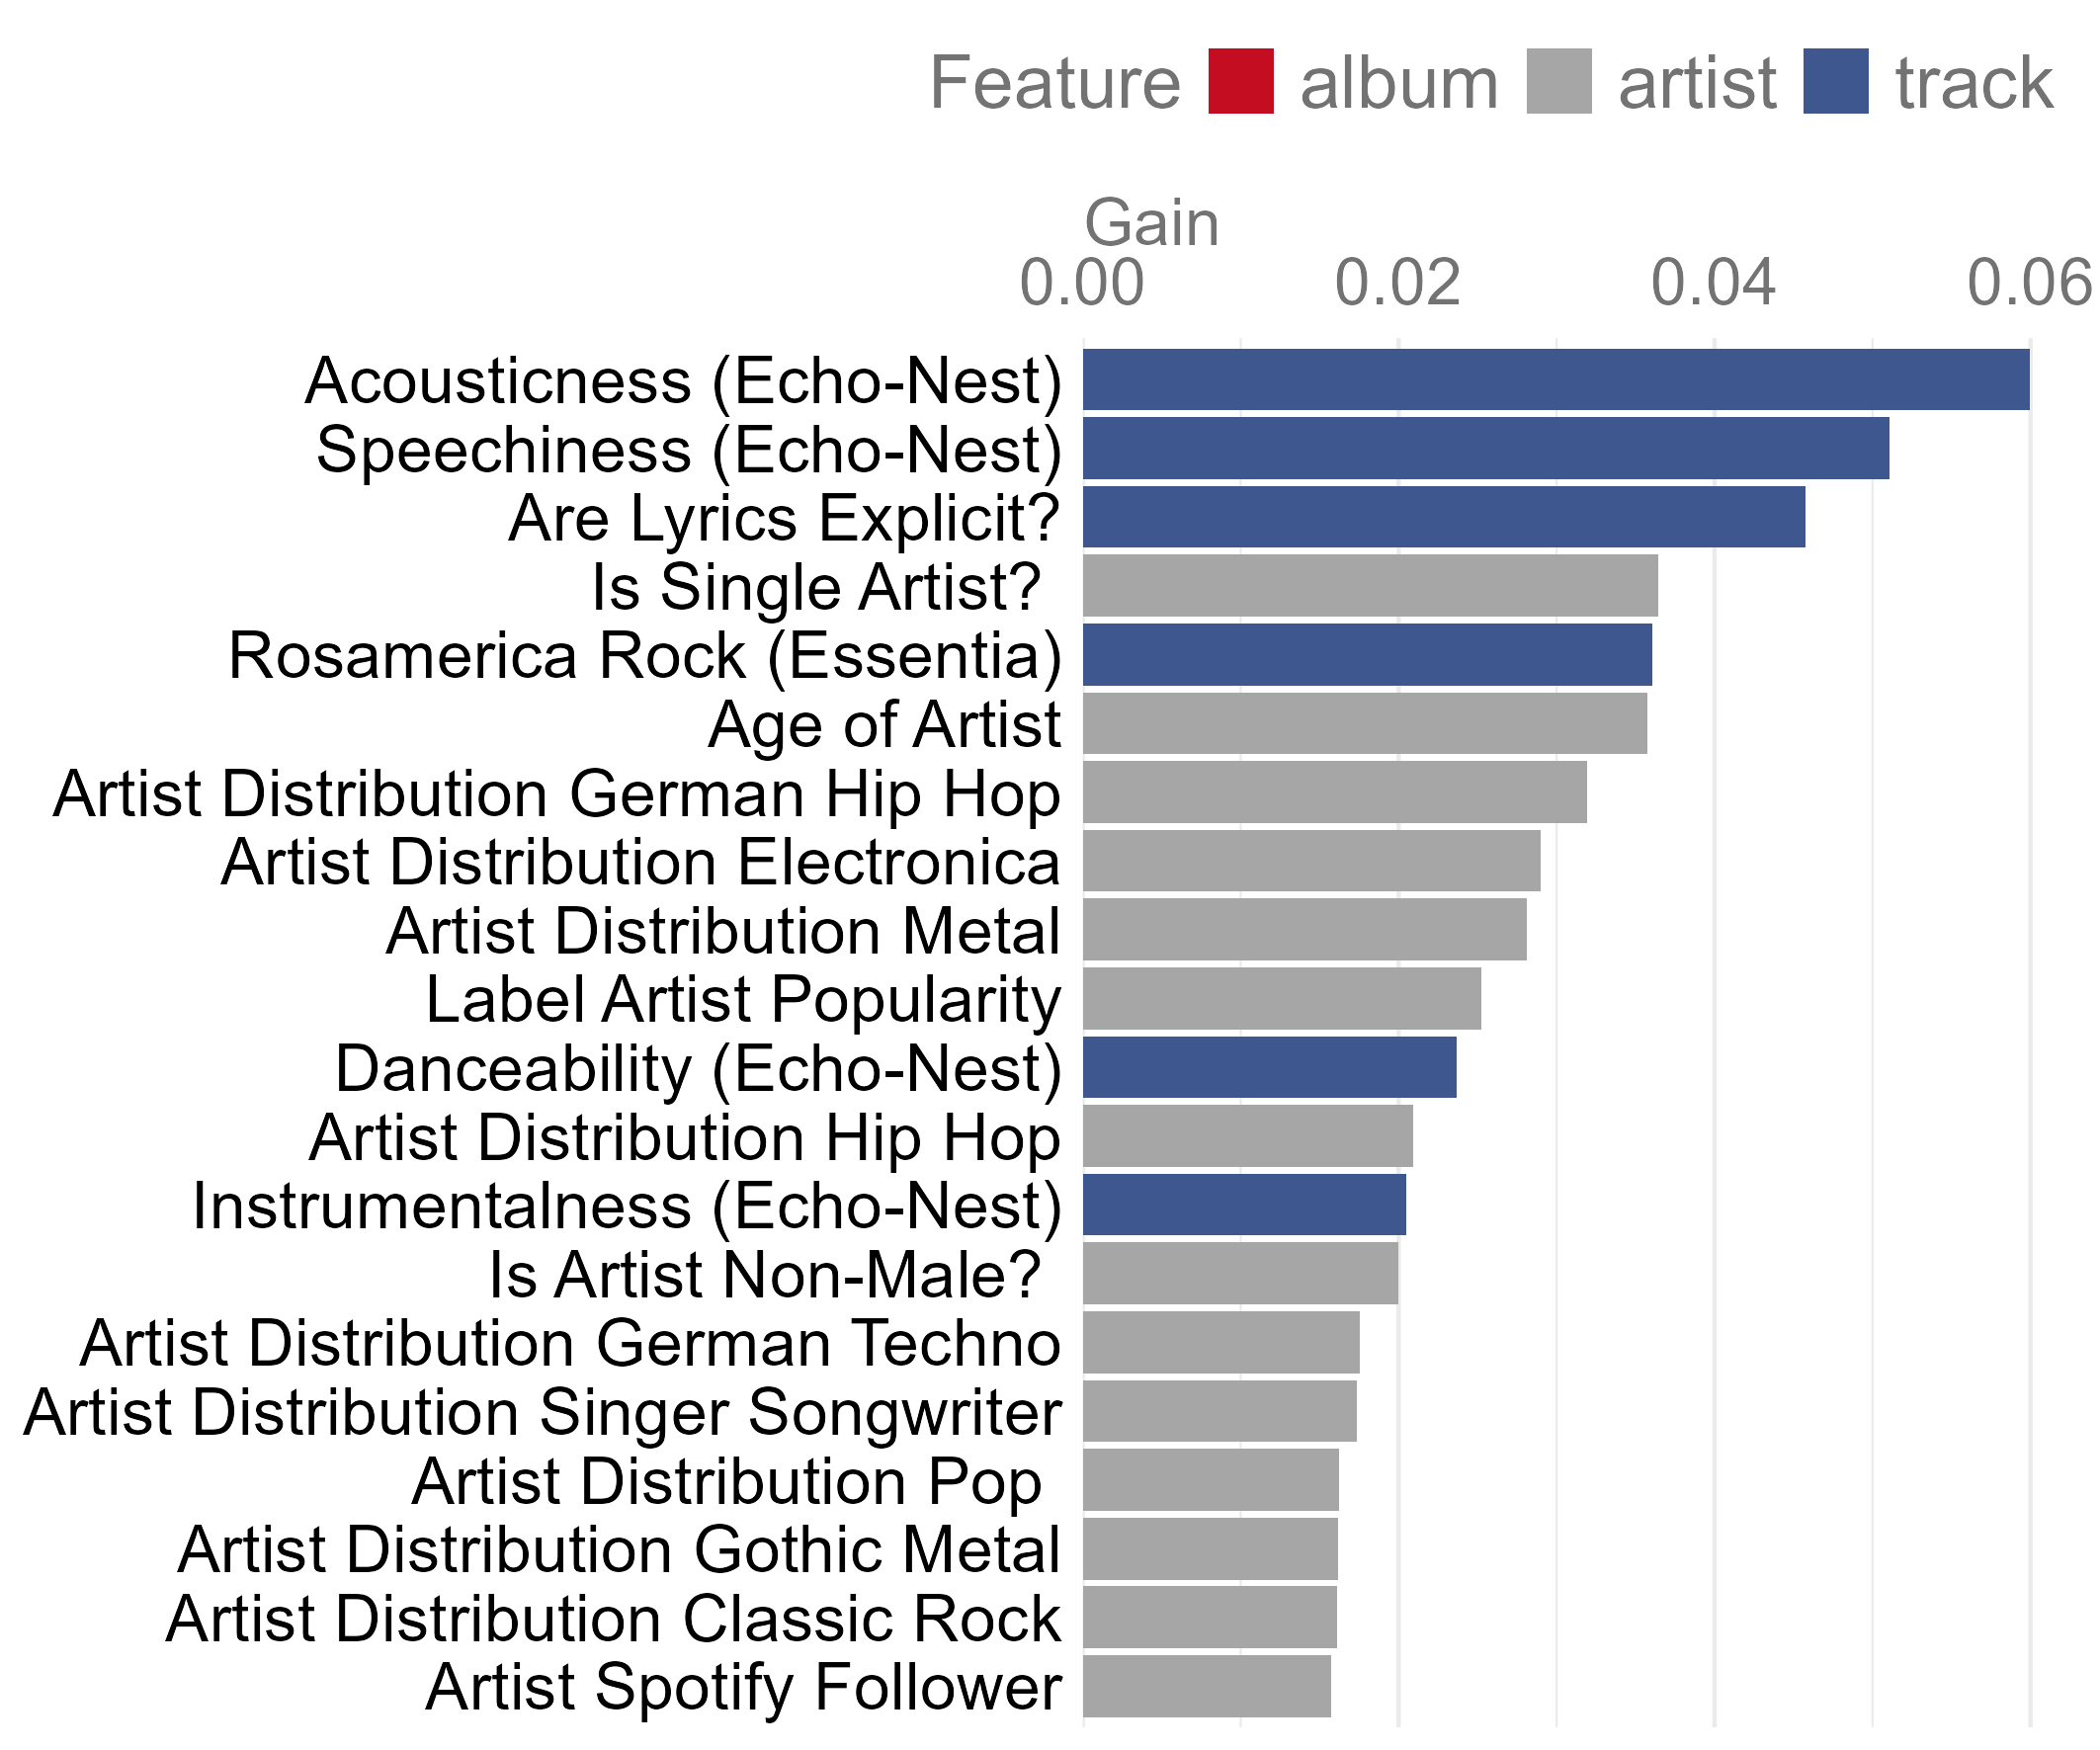
\includegraphics[width=\linewidth]{figures/lightgbm_lowres_varimp.png}
    \caption{COMGET-G5}
    \label{fig:rq3_varimp_low}
  \end{subfigure}
  \hfill
  \vspace{0.25 cm}
  \begin{subfigure}[b]{\columnwidth}
    \centering
    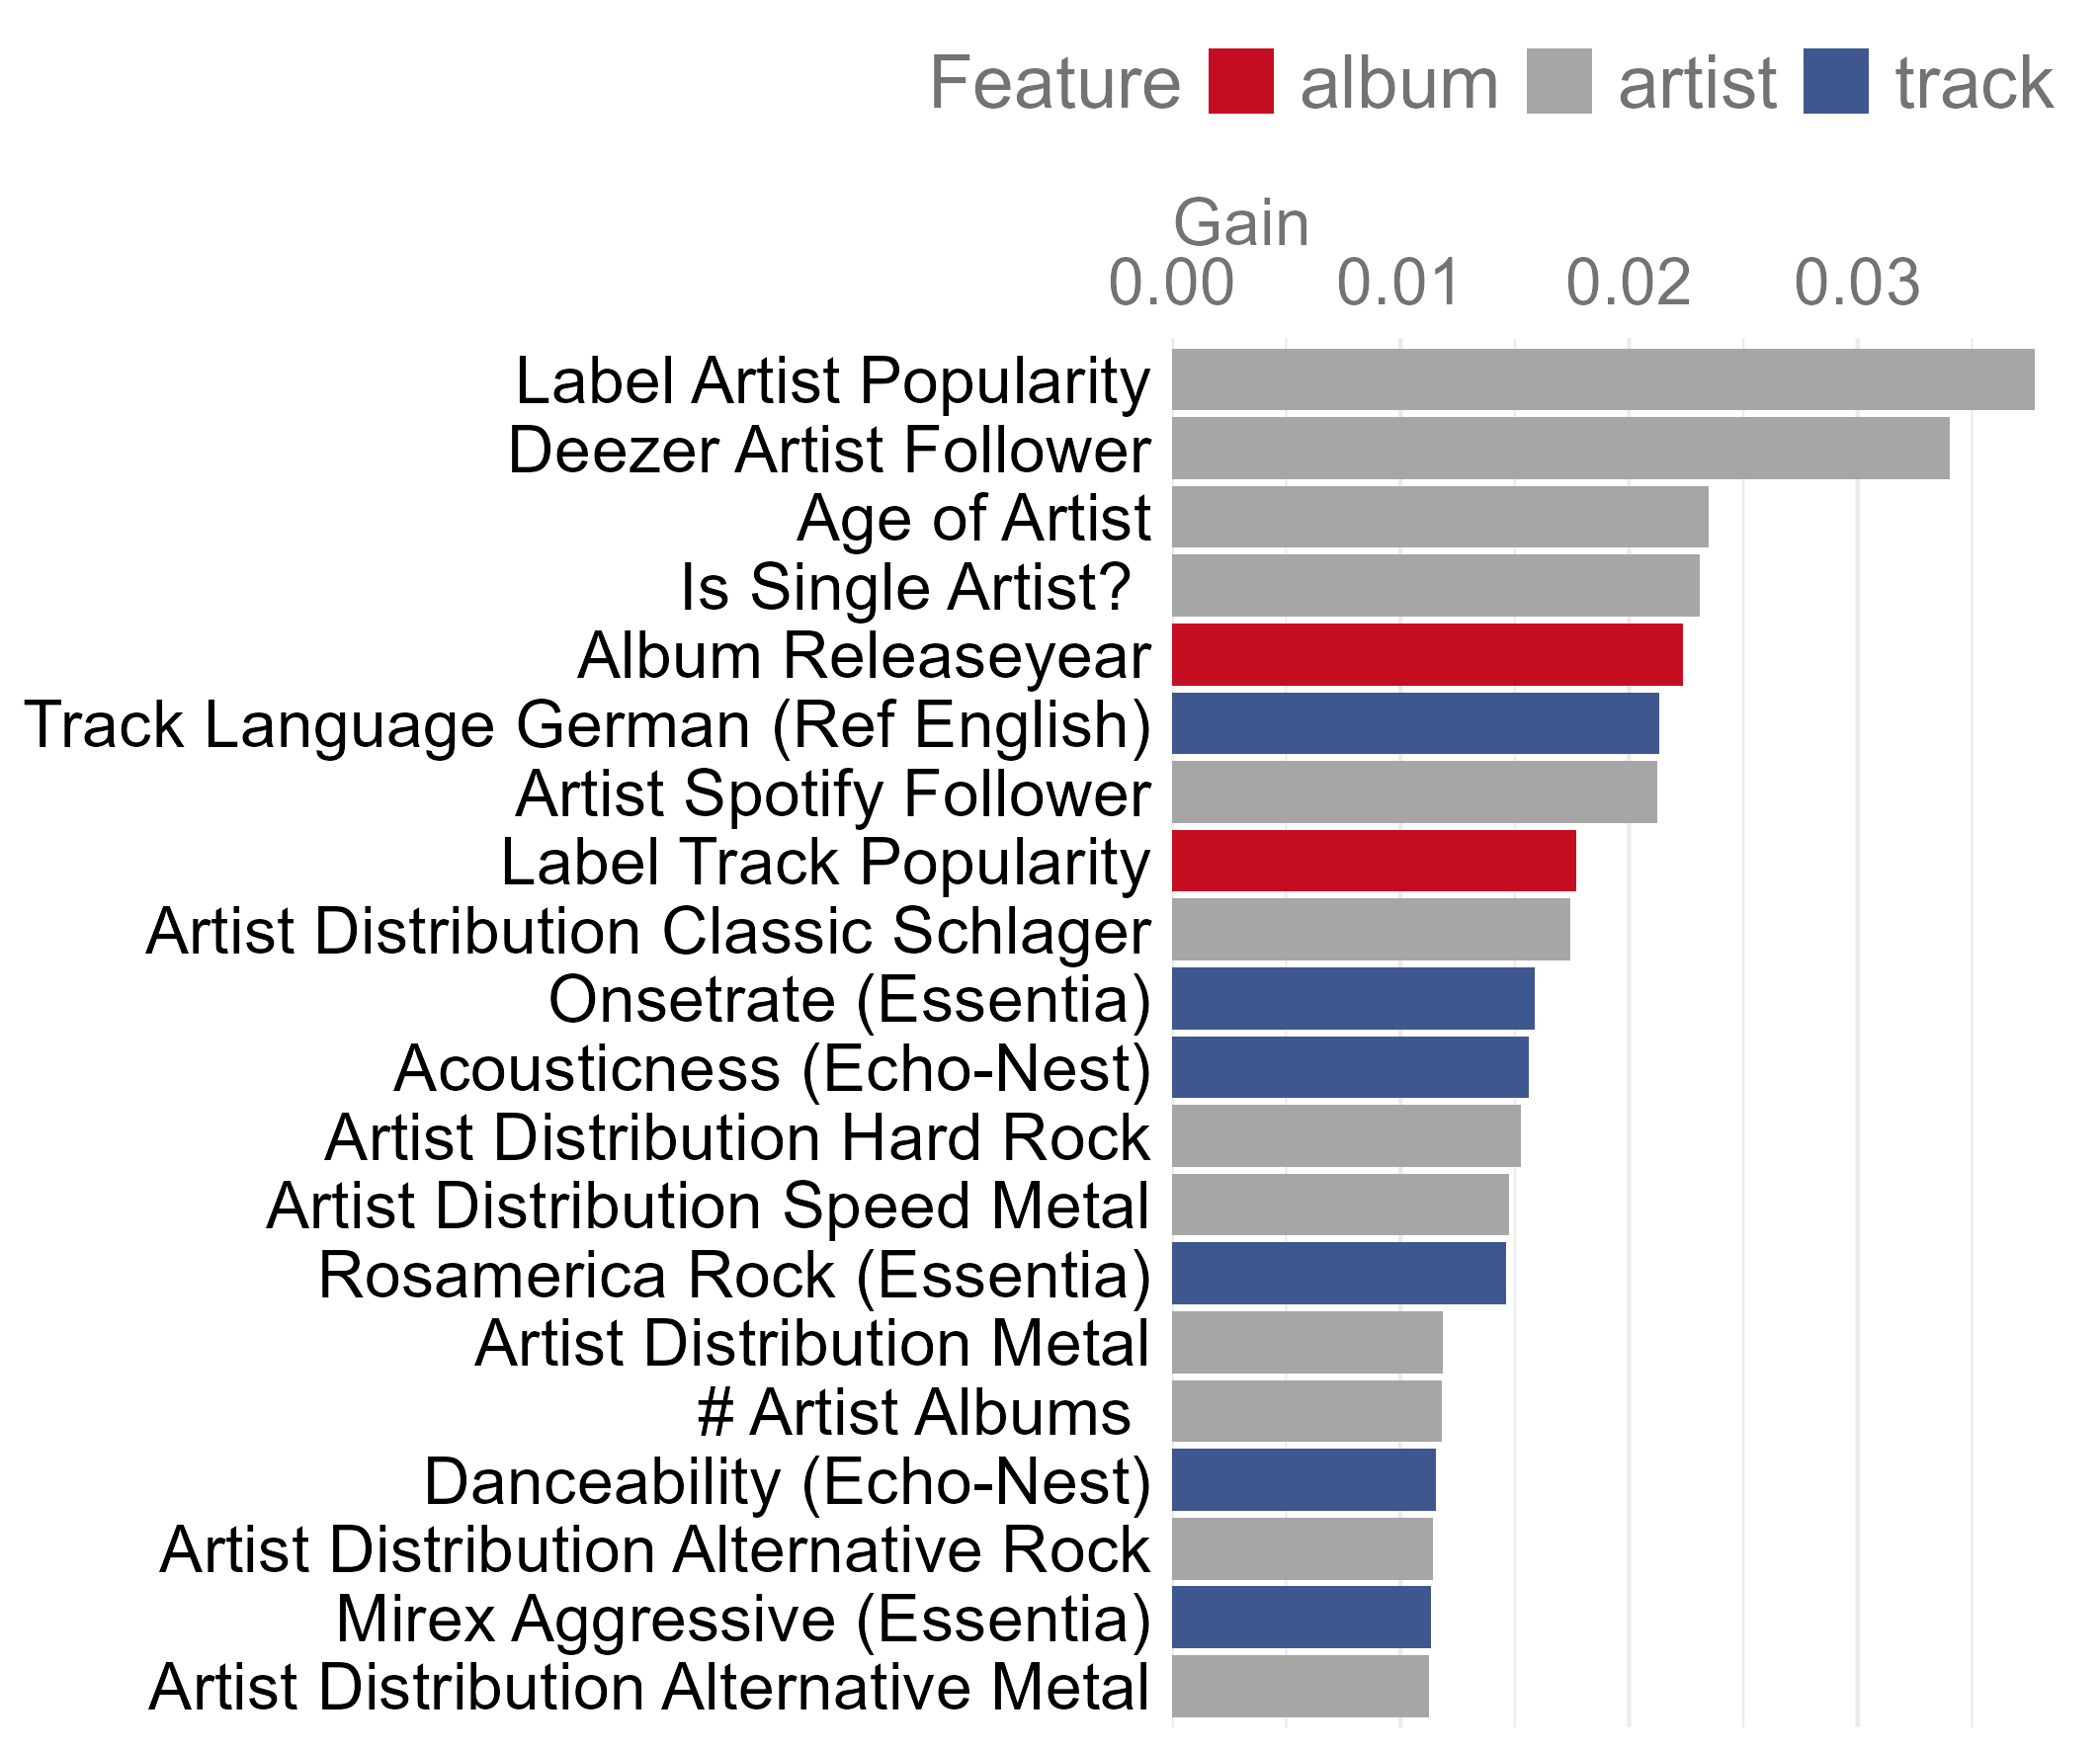
\includegraphics[width=\linewidth, trim={0 0 0 1.5cm}, clip]{figures/lightgbm_mediumres_varimp.png}
    \caption{COMGET-G12}
    \label{fig:rq3_varimp_medium}
  \end{subfigure}
  \caption{Top 20 most important features for automated classification at low and medium granularity. Values show relative feature importance from the final LightGBM models.}
\label{fig:rq3_varimp}
\end{figure}


Figure \ref{fig:rq3_varimp} shows the top 20 most important features for automated classification of COMGET-G5 and COMGET-G12 with the final LightGBM learner (for COMGET-G25 and COMGET-G32 see appendix figure B.2). While we find similar features in the top 20 across all three levels of granularity (e.g., \textit{acousticness (Echo-Nest)}, \textit{artist distributed as ``metal''}, \textit{age of artist}), the importance of single features differs. For COMGET-G5, features that describe general style characteristics (e.g., \textit{acousticness}, \textit{speeciness}, \textit{explicitness of lyrics}) and artist persona (e.g., \textit{single artist vs. band}, \textit{age of artist}) are most important. For COMGET-G12, \textit{popularity} features and the \textit{release year} gain importance. For COMEGET-25G the most important features are mostly artist-related, indicating that fine-grained \textit{genre} distinctions rely primarily on release-milieu signals rather than audio properties.


\section{Discussion}

With the present article, we introduce a novel and methodologically transparent procedure for constructing well-balanced hierarchical genre taxonomies and according genre category assingments from listener-community discourse contained in folksonomies on open music databases. Specifically, we make three key contributions: (1) an algorithm to construct a balanced hierarchical genre tree (COMGET) from folksonomy genre tag co-occurrences, (2) a  folding algorithm (FOLDCAT) that generates optimally balanced hierarchical genre categories and final track-assignments at user-specified granularities from such trees; finally, we (3) demonstrate that resulting community-based genre assignments are a) comparable to existing folkosonomy genre taxonomies (i.e. \textit{Discogs}) and b) can be learned well with supervised machine learning by drawing on openly availiable music descriptors. Hence, our approach can be used as a transparent, reproducible, and empirically grounded alternative to commercial or expert-curated genre taxonomies in future applied or basic research. We demonstrated our approach with a large German popular music corpus (POPTRAG), drawing on \textit{MusicBrainz} folksonomy votes. Nevertheless, the method can in principle be adopted to any other music corpus and other genre tagging systems that provide co-occurences of tags (e.g. \textit{Spotify}, \textit{YouTube}, \textit{SoundCloud}).


\subsection{Benefits for MIR Research and Applications}

A core methodological challenge in MIR stems from genre recognition benchmarks that lack explicit theoretical grounding~\citep{greenCriticalSurveyResearch2024}. Our approach operationalizes genre-as-discourse~\citep{foucaultArchaeologyKnowledge2013, nealeGenre1980}, treating classification as an empirical question rather than an ontological given. This connects computational methods to popular music studies and enables MIR to engage with humanities scholarship on cultural categorization~\citep{dimaggioClassificationArt1987}. 

Furthermore, our single-folksonomy approach ensures epistemic consistency. Mixed-source methods conflate different communities' genre concepts across platforms with varying demographics, tag voting systems, tag pools, and discursive contexts, introducing uncontrolled variance~\citep{schreiberImprovingGenreAnnotations2015,bogdanovAcousticbrainzGenreDataset2019}. Single-source taxonomies eliminate cross-platform variance, ensuring all genre assignments reflect a single community's discourse rather than mixing incompatible categorization systems. Combined with no arbitrary thresholds throughout the pipeline and open-source implementation, this ensures reproducibility and portability to any multi-tag corpus, as demonstrated with \textit{Spotify} distribution genres. Researchers can replicate the method on their target population's folksonomy, generating taxonomies specific to their chosen listener community.

FOLDCAT addresses diverse practical needs while enabling cross-study comparison. The folding algorithm generates optimally balanced genre categories at multiple granularities using a single statistical criterion (Gini coefficient) across hierarchy levels. In addition, the underlying genre category assignments stay probabilistic. Hence, the framework quantifies achievable performance ceilings through community certainty, since models cannot exceed human consistency~\citep{sturmReviewValidityIts2023}. Strong correlations between certainty and classifier performance validate this approach, grounding MIR in listener perception limits. Classifier performance also demonstrates general learnability of the identified genre categories, while systematic confusion patterns reveal fuzzy boundaries (\textit{rock} subgenres), stylistic permeability (\textit{electronic} across \textit{pop}/\textit{jazz}/\textit{indie}), and hierarchical nuance (\textit{heavy metal} versus \textit{metal} asymmetry). These patterns inform which granularities suit different research questions and reaffirm that genre labels remain learnable from the dimensions suggested by the anonymized authors.%Lepa and Radke (2026). 



\subsection{Benefits for Computational Musicology and Cultural Analysis}

COMGET and FOLDCAT consequently implement power-critical concepts from popular music studies and cultural analysis~\citep{dugayDoingCulturalStudies2013} into computational methods for the application on large popular music corpora. Our approach employes democratic aggregation throughout: community votes determine co-occurrences, strongest links define hierarchies, majority voting assigns single labels. Resulting community genre taxonomies, genre categories, and genre category assignments reflect collective hierarchical listener discourse rather than industry or expert impositions, democratizing genre knowledge production for computational musicology. 

Crucially, COMGET taxonomies capture how listeners organize popular music genres in contemporary reception rather than musicological historical genealogies~\citep{pachetTaxonomyMusicalGenres2000}. The POPTRAG demonstration reveals unambiguos genealogical links (\textit{rock} $\rightarrow$ \textit{alternative rock}) alongside counterintuitive ones that invite cultural interpretation rather than genealogical correction. For instance, \textit{classical} and \textit{jazz} emerge as \textit{pop} subgenres. Two factors explain this placement: POPTRAG mostly contains accessible and crossover works—popular opera arias, smooth jazz compilations, chart-oriented classical crossover artists. This corpus profile combines with listeners' tendency to apply broad labels when tagging popular music~\citep{bogdanovAcousticbrainzGenreDataset2019}. Similarly, both \textit{heavy metal} and \textit{metal} appear as \textit{rock} subgenres, reflecting shared historical roots in 1970s psychedelic and hard rock while acknowledging \textit{metal's} later distinctiveness~\citep{gracykHeavyMetalGenre2016}.

Our POPTRAG analysis illustrates the method's capacity to reveal genre discourse structures computationally. \textit{Rock}, \textit{pop}, and \textit{hip hop} emerged as three primary clusters for German popular music genres in Germany, partially aligning with \citet{silverGenreComplexesPopular2016} who identified three main international clusters analyzing MySpace artist networks in 2007. However, structures differ: \textit{rock} forms a distinct cluster in POPTRAG versus Silver et al.'s scattered "Niche" genres; \textit{hip hop} shows minimal differentiation (consistent with Silver et al.); \textit{pop} exhibits stylistic diversity versus Silver et al.'s "Rock 'n Roll" category. Direct comparison remains limited—Silver analyzed artists on a social networking platform, we analyze tracks in a national listening corpus across different decades—yet the method enables such comparative analyses across corpora, revealing how genre discourse varies by platform, national context, and historical period~\citep{pichlMiningCultureSpecificMusic2017,nieInaccuratePredictionGenre2022}. 

Transparent automated classifier analysis reveals how listener communities perceive genres: artist-level features dominate predictions across all granularities in our German popular music analysis, with distribution genre flags (\textit{Spotify} artist tags) and artist demographics outweighing audio features—a finding consistent with genre theory emphasizing release milieu~\citep{nealeGenre1980}. Stylistic features play a secondary role: audio features distinguish broad categories, but bag-of-words and lexical lyric features prove weak, pointing toward LLM-based embeddings as a promising direction~\citep{prevedelloLyricsSuccessEmbedding2024}. Popularity gains importance at finer resolutions as a genre signal itself~\citep{holtGenrePopularMusic2007}. Genre-specific confusion patterns further illuminate boundary strength: e.g., \textit{rock} subgenre overlap (\textit{alternative}, \textit{pop rock}, \textit{indie}) reveals fuzzy boundaries; \textit{electronic} permeability across \textit{pop}, \textit{jazz}, and \textit{indie} reflects stylistic fluidity; and \textit{schlager}–\textit{hip hop} separation demonstrates distinct release milieus and stylistic features.

Beyond cultural research, this method offers new possibilities for stakeholders across the music industry: radio programmers and playlist editors to gain insight into how audiences organize music; A\&R teams to identify gaps between industry positioning and listener reception; marketing departments to recognize which subcultural boundaries audiences perceive versus industry-imposed categories; music journalists to ground critical language in empirical listener consensus; and platform designers to align recommendation logic with listener mental models.

\subsection{Limitations and Future Directions}
Several constraints limit interpretation and generalization of our exemplary results. MusicBrainz launched in 2000 and does not provide individual vote timestamps, so COMGET-G aggregates roughly 25 years of listener votes spanning a period when genre boundaries and perception likely shifted. Platform user demographics and expertise remain opaque (approximately 1.2 million anonymous editor accounts; MusicBrainz,~\citeyear{MusicBrainz_nodate}), preventing assessment of demographic or expertise bias. For the analysis we excluded 36\% of tracks with insufficient votes, thereby introducing slight popularity bias—acceptable for our popular music focus but possibly problematic for niche genres. Methodologically, collinearity among predictors complicates feature importance interpretation. Single-label reduction loses multi-tag nuance, though this simplification proves necessary for many applied research tasks and aligns with our democratic approach.

Future work should pursue three directions. First, convene popular music experts to review the taxonomy, label exemplar tracks for genre categories at different levels of granularity, and identify misassignments to strengthen COMGET-G's validity. Second, replicate the pipeline on independent folksonomies and regional corpora of tracks (e.g., US and UK charts) to reveal how national listening cultures reshape genre structure. Third, enhance classifier prediction through advanced lyric features or learners.



%%%%%%%%%%%%%%%%%%%%%%%%%%%%%%%%%%%%%%%%%%%%%%%%%%%%%%%%%%%%%%%%%%%%%%%%%%%%%%%%
% Please do not touch.
% Print Endnotes
\IfFileExists{\jobname.ent}{
   \theendnotes
}{
   %no endnotes
}
%%%%%%%%%%%%%%%%%%%%%%%%%%%%%%%%%%%%%%%%%%%%%%%%%%%%%%%%%%%%%%%%%%%%%%%%%%%%%%%%

% \section*{Acknowledgements}

% Any acknowledgements must be headed and in a separate paragraph,
% placed after the main text but before the reference list.

%%%%%%%%%%%%%%%%%%%%%%%%%%%%%%%%%%%%%%%%%%%%%%%%%%%%%%%%%%%%%%%%%%%%%%%%%%%%%%%%
% Bibliography
%%%%%%%%%%%%%%%%%%%%%%%%%%%%%%%%%%%%%%%%%%%%%%%%%%%%%%%%%%%%%%%%%%%%%%%%%%%%%%%%

\bibliography{refs}
\end{document}
